%%%%%%%%%%%%%%%%%%%%%%%%%%%%%%%%%%%%%%%%%
% Wenneker Article LaTeX Template Version 2.0 (28/2/17)
%
% This template was downloaded from: http://www.LaTeXTemplates.com
%
% Authors: Vel (vel@LaTeXTemplates.com) Frits Wenneker
%
% License: CC BY-NC-SA 3.0 (http://creativecommons.org/licenses/by-nc-sa/3.0/)
%
%%%%%%%%%%%%%%%%%%%%%%%%%%%%%%%%%%%%%%%%%

%----------------------------------------------------------------------------------------
%	PACKAGES AND OTHER DOCUMENT CONFIGURATIONS
%----------------------------------------------------------------------------------------

\documentclass[10pt, a4paper, twocolumn]{article} % 10pt font size (11 and 12 also possible), A4 paper (letterpaper for US letter) and two column layout (remove for one column)

%%%%%%%%%%%%%%%%%%%%%%%%%%%%%%%%%%%%%%%%%
% Wenneker Article
% Structure Specification File
% Version 1.0 (28/2/17)
%
% This file originates from:
% http://www.LaTeXTemplates.com
%
% Authors:
% Frits Wenneker
% Vel (vel@LaTeXTemplates.com)
%
% License:
% CC BY-NC-SA 3.0 (http://creativecommons.org/licenses/by-nc-sa/3.0/)
%
%%%%%%%%%%%%%%%%%%%%%%%%%%%%%%%%%%%%%%%%%

%----------------------------------------------------------------------------------------
%	PACKAGES AND OTHER DOCUMENT CONFIGURATIONS
%----------------------------------------------------------------------------------------

\usepackage[english]{babel} % English language hyphenation

\usepackage{microtype} % Better typography

\usepackage{amsmath,amsfonts,amsthm} % Math packages for equations

\usepackage[svgnames]{xcolor} % Enabling colors by their 'svgnames'

\usepackage[hang, small, labelfont=bf, up, textfont=it]{caption} % Custom captions under/above tables and figures

\usepackage{booktabs} % Horizontal rules in tables

\usepackage{lastpage} % Used to determine the number of pages in the document (for "Page X of Total")

\usepackage{graphicx} % Required for adding images

\usepackage{enumitem} % Required for customising lists
\setlist{noitemsep} % Remove spacing between bullet/numbered list elements

\usepackage{sectsty} % Enables custom section titles
\allsectionsfont{\usefont{OT1}{phv}{b}{n}} % Change the font of all section commands (Helvetica)

\usepackage{amsmath} % Allows for mathematical symbols
\usepackage{mdframed} % Allows for framing of text

%----------------------------------------------------------------------------------------
%	MARGINS AND SPACING
%----------------------------------------------------------------------------------------

\usepackage{geometry} % Required for adjusting page dimensions

\geometry{
	top=1cm, % Top margin
	bottom=1.5cm, % Bottom margin
	left=2cm, % Left margin
	right=2cm, % Right margin
	includehead, % Include space for a header
	includefoot, % Include space for a footer
	%showframe, % Uncomment to show how the type block is set on the page
}

\setlength{\columnsep}{2.5mm} % Column separation width

\setlength{\parskip}{2.5mm} % Increase spacing between paragraphs

%----------------------------------------------------------------------------------------
%	FONTS
%----------------------------------------------------------------------------------------

\usepackage[T1]{fontenc} % Output font encoding for international characters
\usepackage[utf8]{inputenc} % Required for inputting international characters

\usepackage{XCharter} % Use the XCharter font

%----------------------------------------------------------------------------------------
%	HEADERS AND FOOTERS
%----------------------------------------------------------------------------------------

\usepackage{fancyhdr} % Needed to define custom headers/footers
\pagestyle{fancy} % Enables the custom headers/footers

\renewcommand{\headrulewidth}{0.0pt} % No header rule
\renewcommand{\footrulewidth}{0.4pt} % Thin footer rule

\renewcommand{\sectionmark}[1]{\markboth{#1}{}} % Removes the section number from the header when \leftmark is used

%\nouppercase\leftmark % Add this to one of the lines below if you want a section title in the header/footer

% Headers
\lhead{} % Left header
\chead{\fontfamily{phv}\selectfont\textit{\thetitle}} % Center header - currently printing the article title
\rhead{} % Right header

% Footers
\lfoot{} % Left footer
\cfoot{} % Center footer
\rfoot{\fontfamily{phv}\selectfont\footnotesize Page \thepage\ of \pageref{LastPage}} % Right footer, "Page 1 of 2"

\fancypagestyle{firstpage}{ % Page style for the first page with the title
	\fancyhf{}
	\renewcommand{\footrulewidth}{0.0pt} % Suppress footer rule
}

\makeatletter{}
\renewcommand{\thepage}{\textsf{\@arabic\c@page}}
\makeatother{}

%----------------------------------------------------------------------------------------
%	TITLE SECTION
%----------------------------------------------------------------------------------------

\definecolor{tudublinblue}{HTML}{004C6C}

\newcommand{\authorstyle}[1]{{\large\usefont{OT1}{phv}{b}{n}\color{tudublinblue}#1}} % Authors style (Helvetica)

\newcommand{\institution}[1]{{\footnotesize\usefont{OT1}{phv}{m}{sl}\color{Black}#1}} % Institutions style (Helvetica)

\usepackage{titling} % Allows custom title configuration

\newcommand{\HorRule}{\color{DarkGrey}\rule{\linewidth}{1pt}} % Defines the gold horizontal rule around the title

\pretitle{
	\vspace{-30pt} % Move the entire title section up
	\HorRule\vspace{10pt} % Horizontal rule before the title
	\fontsize{32}{36}\usefont{OT1}{phv}{b}{n}\selectfont % Helvetica
	\color{tudublinblue} % Text colour for the title and author(s)
}

\posttitle{\par\vskip 15pt} % Whitespace under the title

\preauthor{} % Anything that will appear before \author is printed

\postauthor{ % Anything that will appear after \author is printed
	\vspace{10pt} % Space before the rule
	\par\HorRule % Horizontal rule after the title
	\vspace{20pt} % Space after the title section
}



%----------------------------------------------------------------------------------------
%	TABLE OF CONTENTS
%----------------------------------------------------------------------------------------

\usepackage{tocloft}



% fonts for TOC
\renewcommand{\cfttoctitlefont}{\fontfamily{phv}\selectfont\Large\bfseries}
\renewcommand{\cftsecfont}{\fontfamily{phv}\selectfont\bfseries}
\renewcommand{\cftsecpagefont}{\fontfamily{phv}\selectfont}
\renewcommand{\cftsubsecfont}{\fontfamily{phv}\selectfont\itshape}
\renewcommand{\cftsubsecpagefont}{\fontfamily{phv}\selectfont}

\renewcommand{\cftloftitlefont}{\fontfamily{phv}\selectfont\Large\bfseries} % List of Figures title
\renewcommand{\cftlottitlefont}{\fontfamily{phv}\selectfont\Large\bfseries} % List of Tables title

\setcounter{tocdepth}{3}


%----------------------------------------------------------------------------------------
%	ABSTRACT
%----------------------------------------------------------------------------------------

\usepackage{lettrine} % Package to accentuate the first letter of the text (lettrine)
\usepackage{fix-cm}	% Fixes the height of the lettrine

\newcommand{\initial}[1]{ % Defines the command and style for the lettrine
	\lettrine[lines=3,findent=4pt,nindent=0pt]{% Lettrine takes up 3 lines, the text to the right of it is indented 4pt and further indenting of lines 2+ is stopped
		\color{DarkGoldenrod}% Lettrine colour
		{#1}% The letter
	}{}%
}

\usepackage{xstring} % Required for string manipulation

\newcommand{\lettrineabstract}[1]{
	\StrLeft{#1}{1}[\firstletter] % Capture the first letter of the abstract for the lettrine
	\initial{\firstletter}\textbf{\StrGobbleLeft{#1}{1}} % Print the abstract with the first letter as a lettrine and the rest in bold
}

%----------------------------------------------------------------------------------------
%	BIBLIOGRAPHY
%----------------------------------------------------------------------------------------

\usepackage[backend=bibtex,style=authoryear,natbib=true]{biblatex} % Use the bibtex backend with the authoryear citation style (which resembles APA)

\addbibresource{sources.bib} % The filename of the bibliography

\usepackage[autostyle=true]{csquotes} % Required to generate language-dependent quotes in the bibliography
 % Specifies the document structure and loads requires packages

%----------------------------------------------------------------------------------------
%	ARTICLE INFORMATION
%----------------------------------------------------------------------------------------

\title{Group 3: Interim Report} % The article title

\author{
	\authorstyle{
		Saul Burgess - C19349793 --- Andreas Kraus - D23125112 \\
		Kaustubh Trivedi - D23124940 --- Jessica Fornetti - D23124588 \\
		Anais Blenet - D22127697 --- Yuanshuo Du - D22125495
		} % Authors
}

% Example of a one line author/institution relationship
%\author{\newauthor{John Marston} \newinstitution{Universidad Nacional Autónoma de México, Mexico City, Mexico}}

\date{\today} % Add a date here if you would like one to appear underneath the title block, use \today for the current date, leave empty for no date

%----------------------------------------------------------------------------------------

\begin{document}

\maketitle % Print the title

\thispagestyle{firstpage} % Apply the page style for the first page (no headers and footers)

%----------------------------------------------------------------------------------------
%	ARTICLE CONTENTS
%----------------------------------------------------------------------------------------

\section{User Scenario:}
\documentclass[preview]{standalone}
\begin{document}

\subsection{Who is our target user?}
\textit{Magpie's} primary target is Urban Planners. Urban Planners are
professionals responsible for the development of cities and towns, focusing on
the efficient use of land, infrastructure planning, and the creation of
sustainable and resilient communities. (\cite{fischler2012fifty}) Our secondary
target is any casual user who is interested in amenities planning, and this
includes but is not limited to the following: Sustainability Advocates,
Commuters, Event Planners, Journalists, Political Advisors, and Parking
Companies.

These personas were developed on basis of a combination of real-life people who
are known to our team, as well as based on research into the goals and needs of
people in these professions

\subsubsection{Primary Persona - Michael O'Brien}
O'Brien is a 48-year-old Urban Planning Specialist at Dublin City Council,
deeply committed to enhancing his hometown of Lusk. He specializes in
sustainable urban development, integrating smart technologies with traditional
planning principles, and has contributed to notable projects like Dublin's cycle
lane network. He represents our primary target user.

Michael is currently working on the expansion of Dublin's cycle lane network
southbound. He is facing some challenges because the maps provided by Dublin
city council are static and don't show crucial information such as public
facilities and amenities. The datasets he's been accessing seem out of date and
not comprehensive at all. Michael needs a tool that allows him to interact with
a map that contains key data on public facilities and amenities, as well as
options to extract that information for analysis and planning.

%michael user persona
\begin{figure}[htbp]
    \centering{}{}
    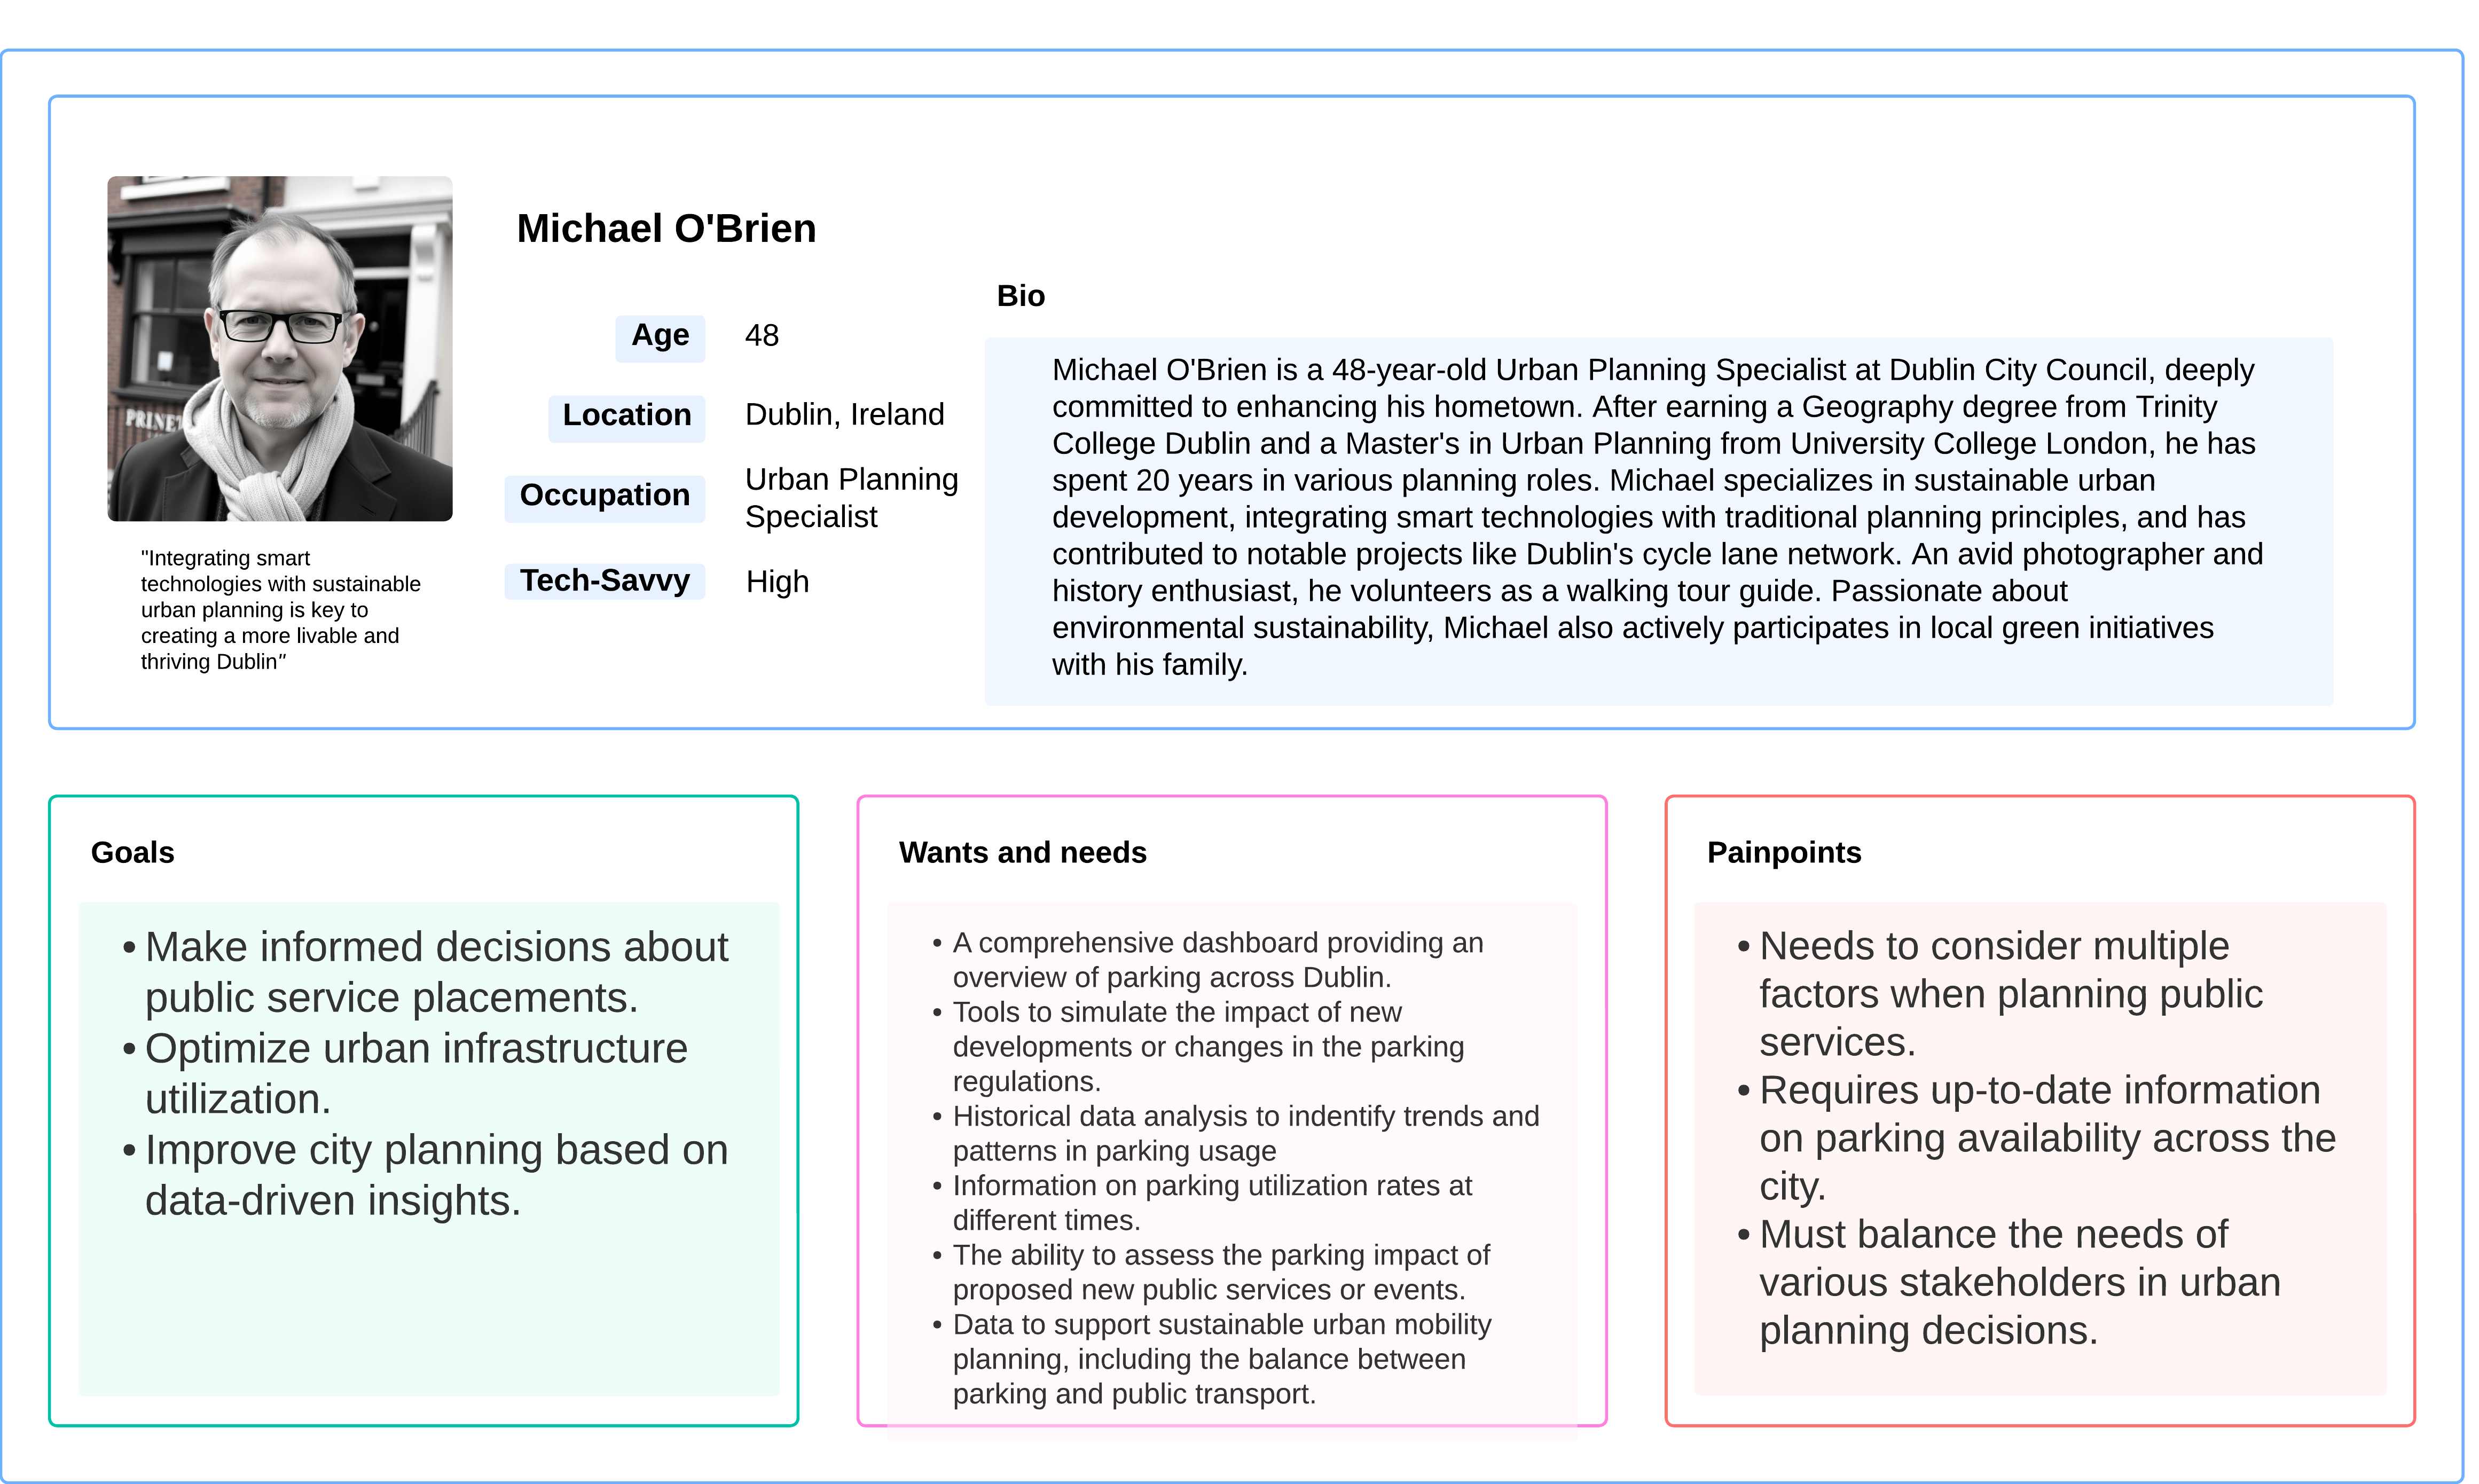
\includegraphics[width=0.8\textwidth]{images/michael-obrien-userpersona.png}
    \caption{User persona - Michael O'Brien}
\end{figure}

\subsubsection{Secondary Persona - Sarah Thompson}
Sarah thompson is a 35 year old CEO of an event's planning company based in
Dublin, Ireland. She specializes in corporate events and weddings, and is known
for creating memorable experiences while addressing key logistical challenges
such as venue selection, catering, accessibility and transportation. She
represents our secondary target user.

%sarah user persona
\begin{figure}[htbp!]
    \centering{}{}
    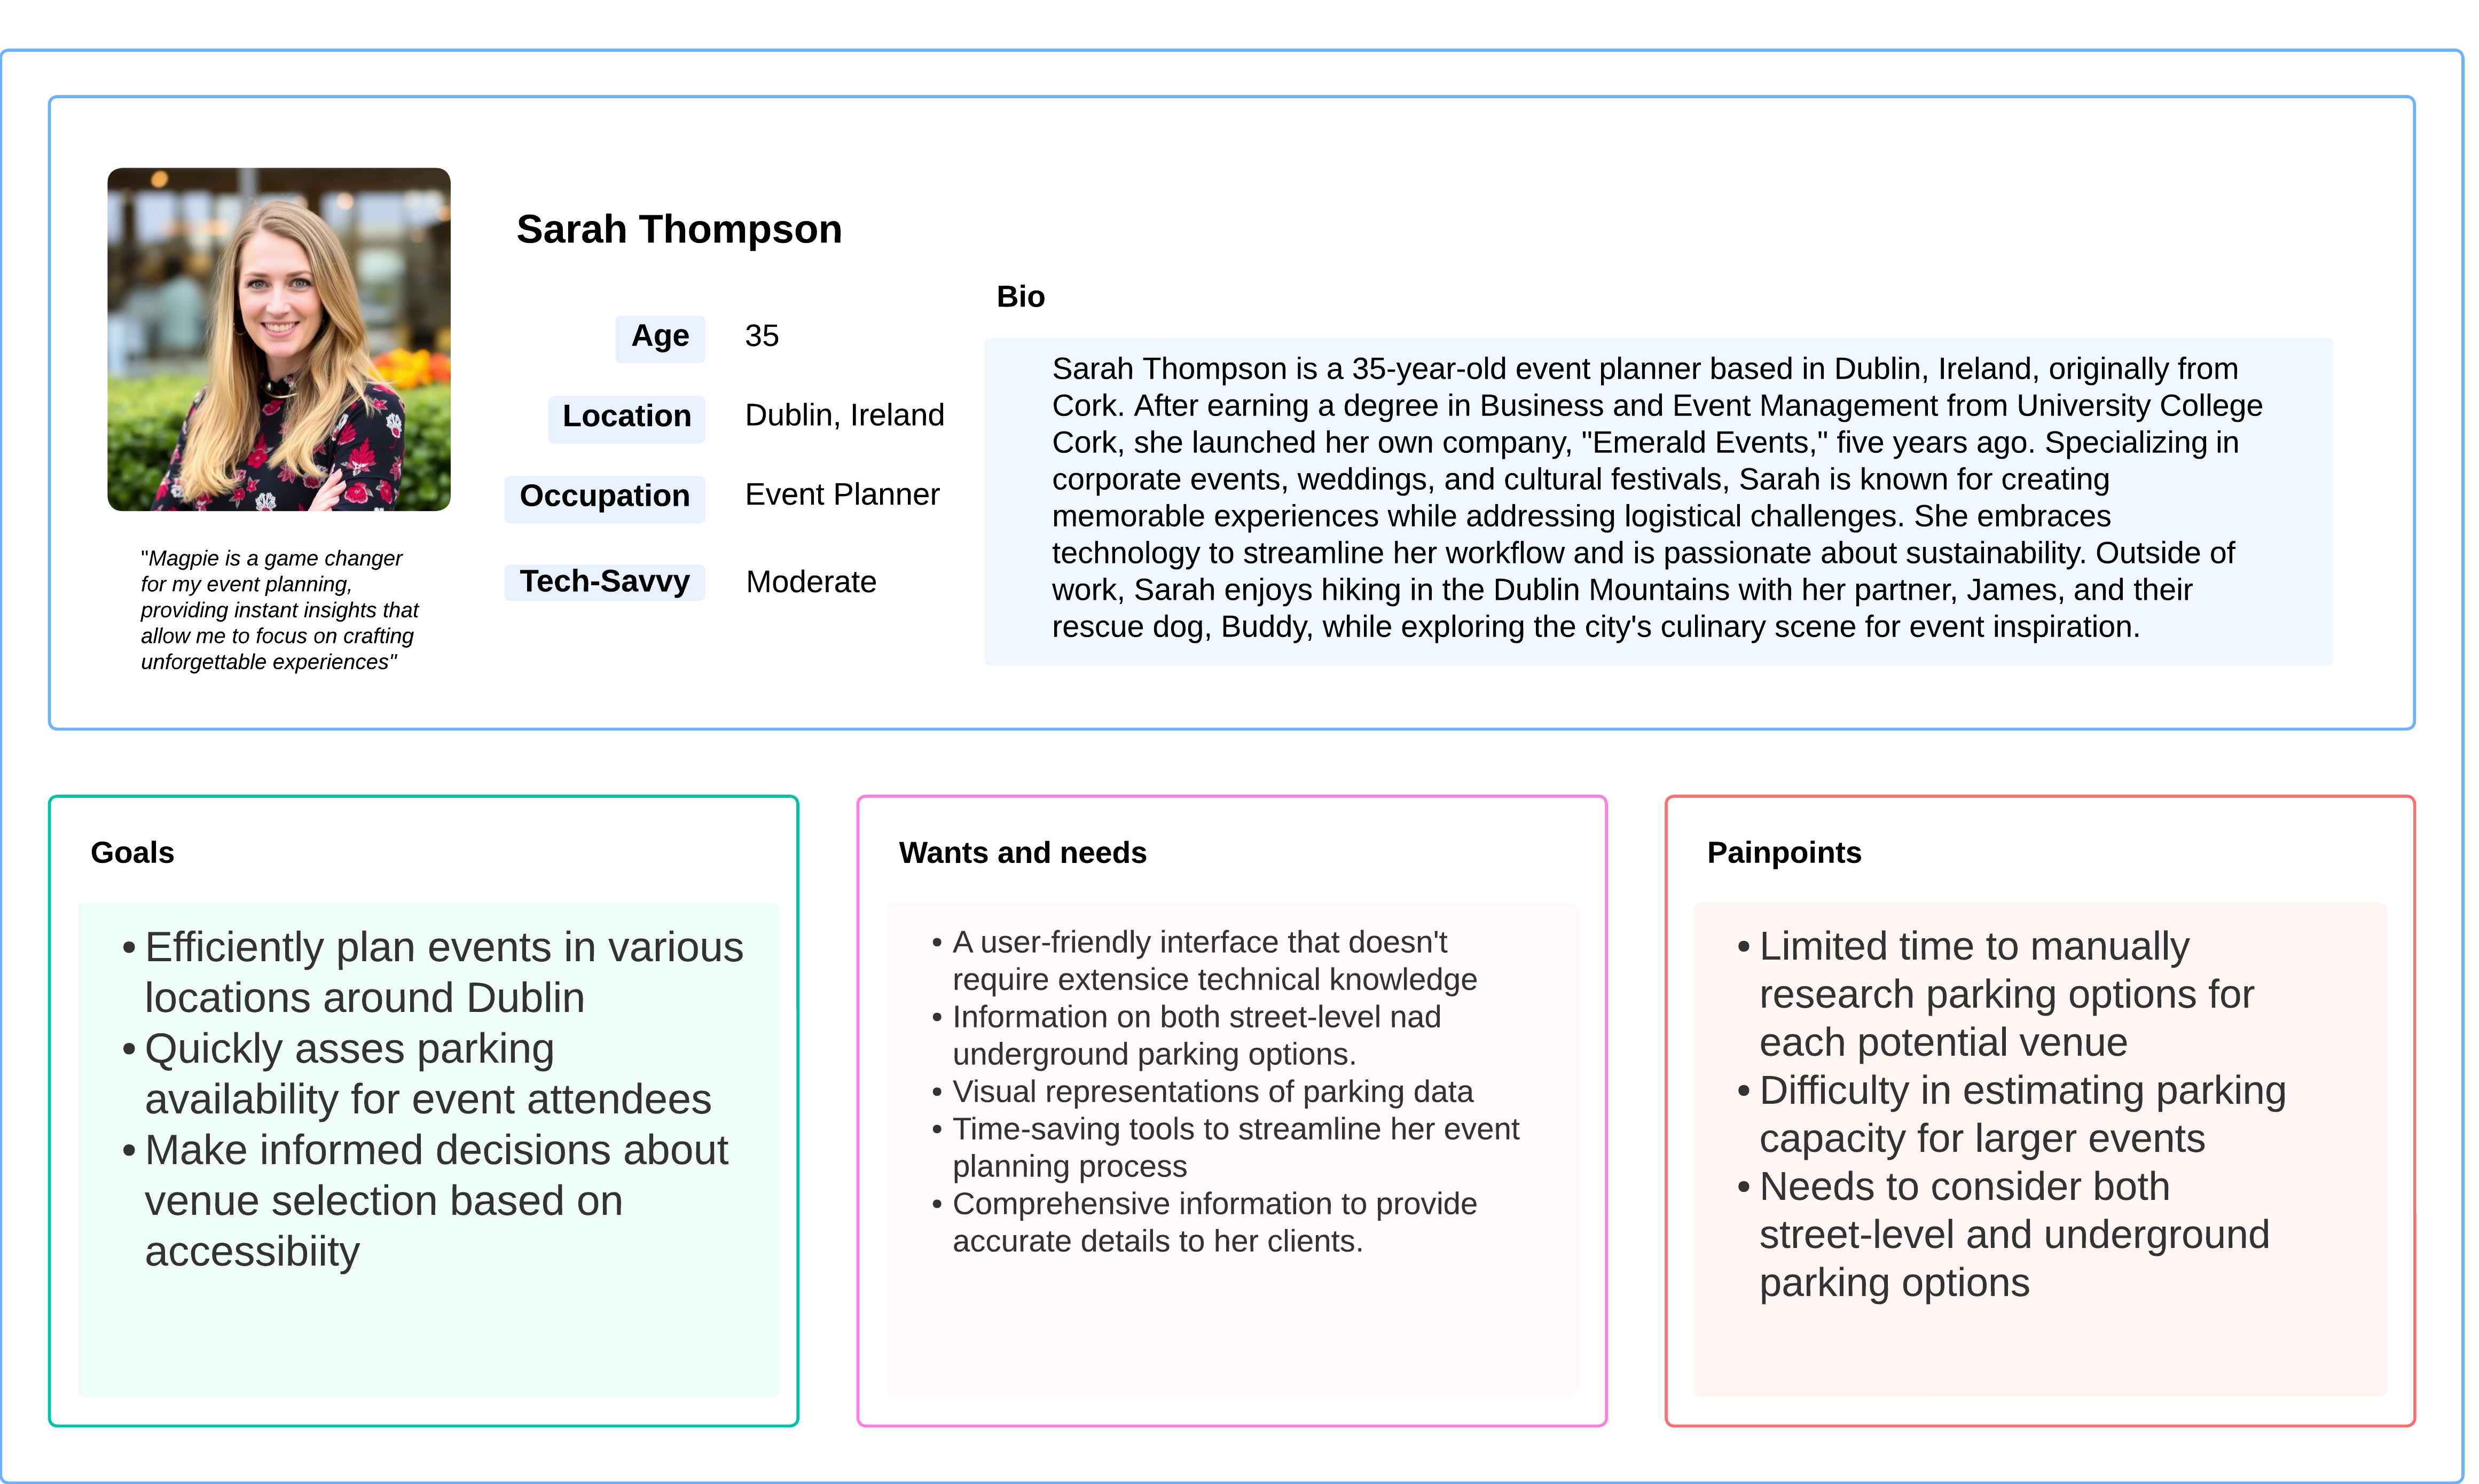
\includegraphics[width=0.8\textwidth]{images/sarah-thompson-userpersona.png}
    \caption{User persona - Sarah Thompson}
\end{figure}

\newpage{}

Currently, she faces many challenges planning events within Dublin city. She has
limited time to manually research transport and parking options and to visually
assess the accessibility of a possible venue. She's looking for a tool that will
give her a visual overview of transportation and parking options in an area,
with additional information on their location  \& their quantity. She also needs
something quick and easy to use.

\subsection{Why are they important?}
Urban Planners are crucial for the holistic development of cities and towns.
(\cite{jha2021review})They ensure that urban development is sustainable,
balancing economic growth and environmental protection. (\cite{lei2021urban})
Urban planners guide cities towards more efficient uses of land, better
transport systems, and overall increasing the quality of life of residents.
(\cite{janpavle2022importance})

By planning for current and future needs, Urban Planners help mitigate urban
challenges such as congestion, pollution, and lack of infrastructure. Their role
is essential for ensuring that urban areas can meet the demands of growing
populations, while maintaining standard of living and environmental
sustainability.

\subsection{What problem are we solving?}
Urban Planners often face challenges with accessing and analysing data. Data is
typically siloed, making it difficult to access and analyse.
(\cite{duivenvoorden2021managing})

We aim to provide Urban Planners with a tool that allows them to access this
information in a single, easy to use, platform. This will allow Urban Planners
to streamline the initial phases of their work, decreasing the time spent on
data collection and increasing the time spent on analysis and decision making.

\subsection{Market analysis}
The identification of our target user was made possible through exploratory work
done at the beginning of the project timeline. A research survey was conducted
using Microsoft Forms, sent out to county councils, planners, firms and the
TUDublin mailing list, to answer key demographic \& product questions:
\begin{enumerate}
    \item{Who is our primary target user?}
    \item{What kind of amenity data do they access and how?}
    \item{What devices/tools do they primarily use?}
    \item{Are they satisfied with those tools?}
    \item{Would they consider Magpie useful in filling the gaps in their toolset?}
\end{enumerate}

\newpage{}

\subsubsection{Demographic data}
This first section of the survey covered demographic data, to allow us to build a profile for the respondents. Personal identifiable information was not collected for the purposes of anonymity.

We had a total of 118 respondents, which we divided into 2 categories:

\emph{User A}: Respondents who did not use amenity data in their work = \textbf{88 users}.
\emph{User B}: Respondents who used amenity data in their work = \textbf{30 users}.
Splitting the respondents allows us to better analyse the answers in the context of if they belong to our primary or our secondary target user group.

Both user groups were evenly distributed in employment sector and counties they work in, as illustrated in the figures below.

%user sector distribution
\begin{figure}[htbp]
    \centering{}{}
    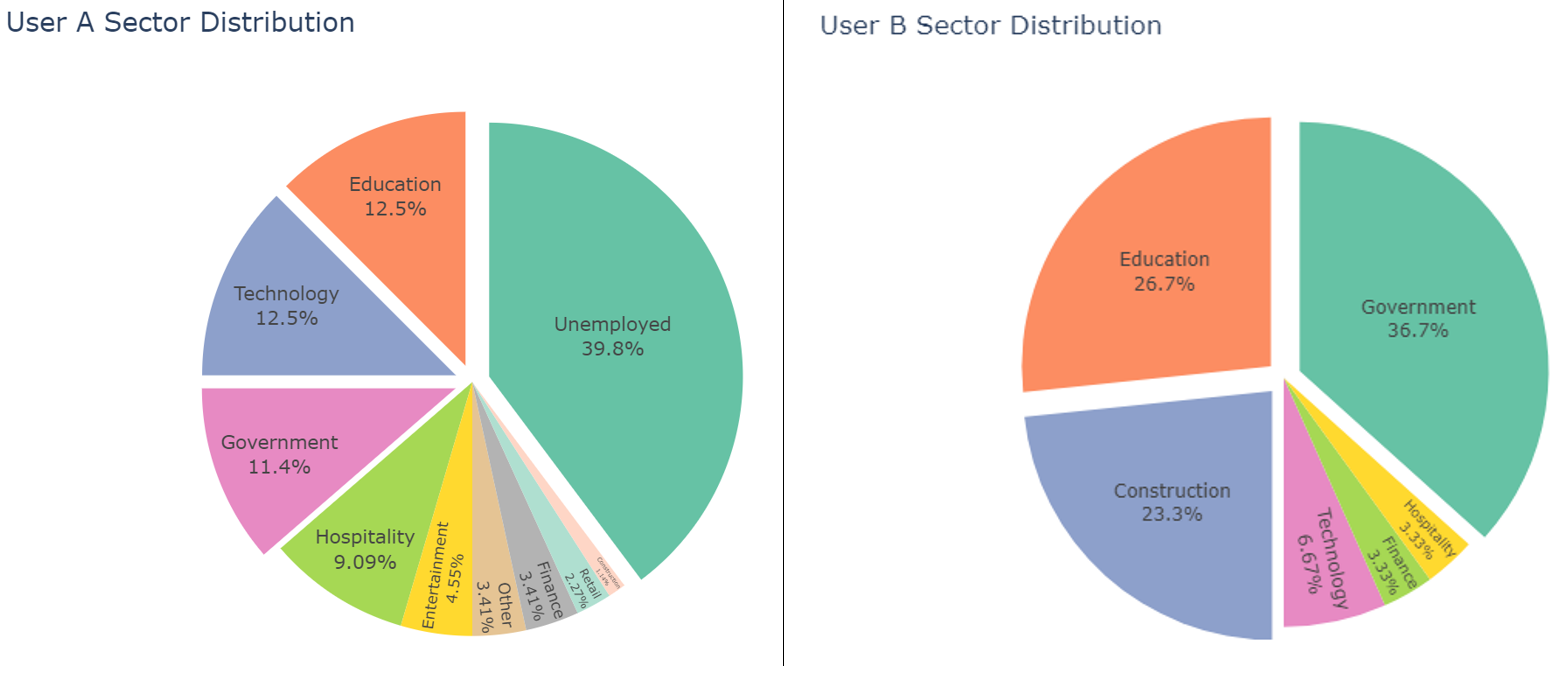
\includegraphics[width=0.8\textwidth]{images/mr-sector-distribution.png}
    \caption{Market analysis - User Sector Distribution}
\end{figure}

%user sector distribution
\begin{figure}[htbp]
    \centering{}{}
    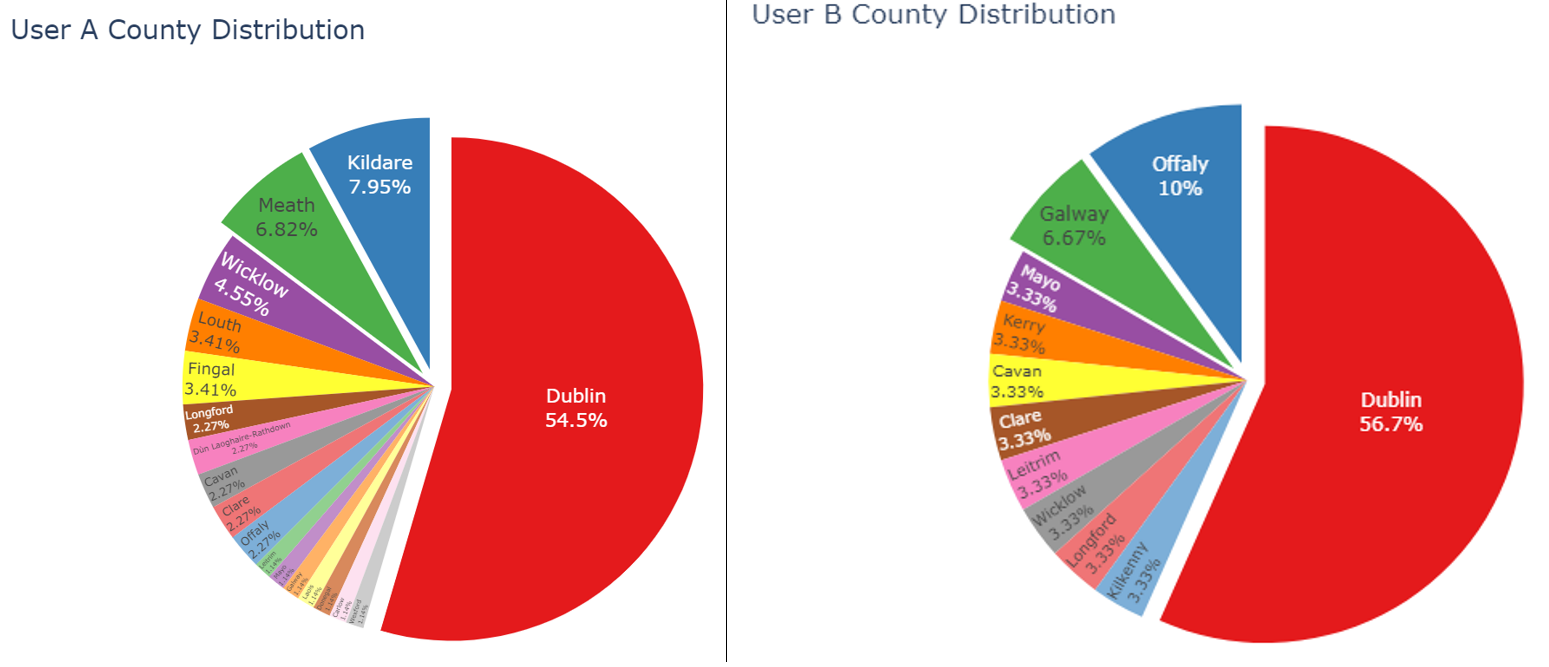
\includegraphics[width=0.8\textwidth]{images/mr-county-distribution.png}
    \caption{Market analysis - User County Distribution}
\end{figure}

\newpage{}

\subsubsection{Amenity data}
This section specifically questions respondents in the User B group on their use of amenity data in their work.

We can see that the most common amenity data accessed is transportation.

%amenity data type accessed
\begin{figure}[htbp]
    \centering{}{}
    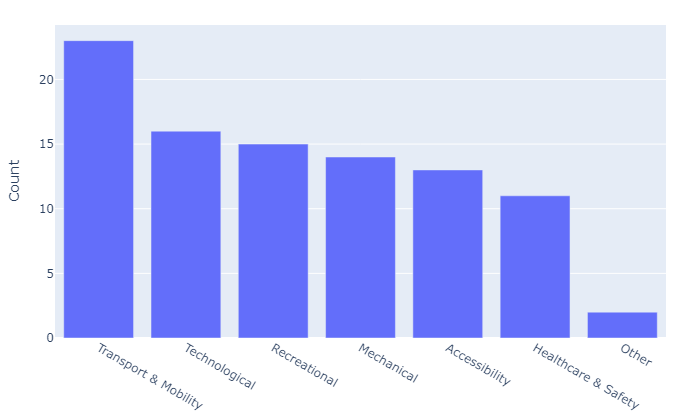
\includegraphics[width=0.8\textwidth]{images/mr-userb-amenity.png}
    \caption{Market analysis - User B Amenity Data Type Distribution}
\end{figure}

\subsubsection{Devices \& Tools}
This section looks at the devices used by both users groups, as well as the
applications or tools they are using to access amenity data.

User A was specifically questioned on which device they use for navigation and
at what frequency.

%device + freq user A
\begin{figure}[htbp]
    \centering{}{}
    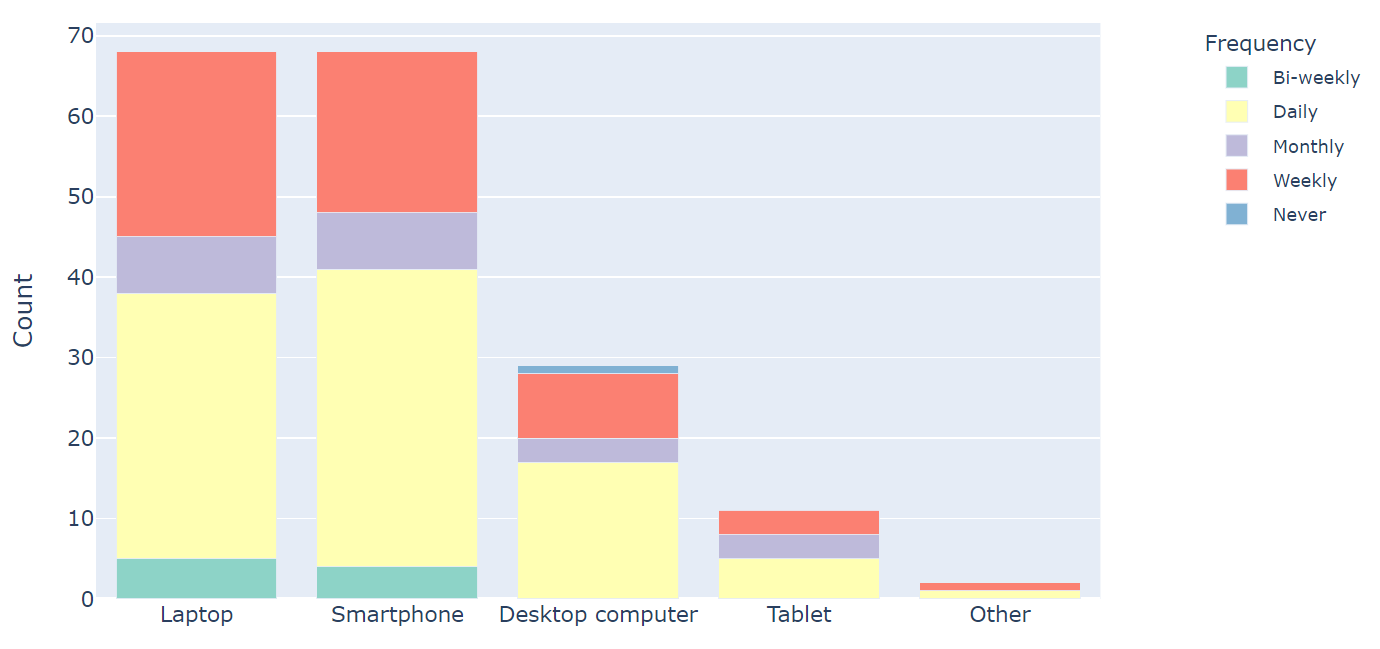
\includegraphics[width=0.8\textwidth]{images/mr-usera-device-freq.png}
    \caption{Market analysis - User A Preferred device \& Usage frequency}
\end{figure}

User B was specifically questioned on which device they use for their day-to-day
work, as well as what tool they are currently using to access amenity data.

%device + freq user B
\begin{figure}[htbp]
    \centering{}
    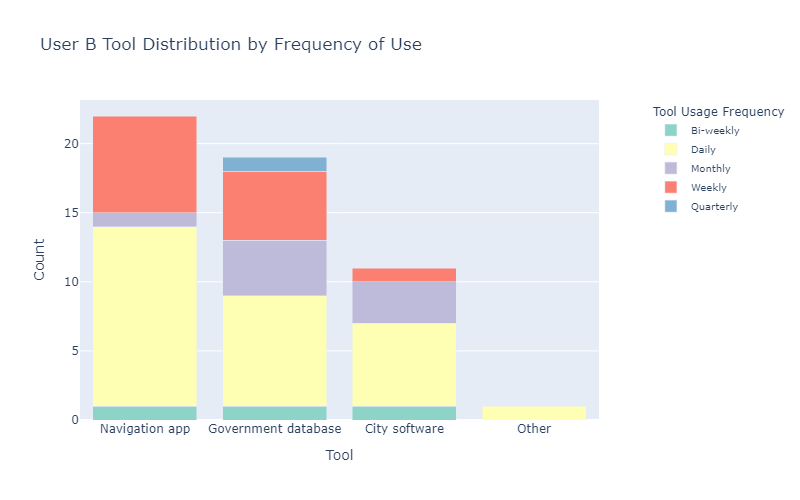
\includegraphics[width=0.8\textwidth]{images/mr-userb-tool-freq.png}
    \caption{Market analysis - User B Tool type \& Usage frequency}
\end{figure}

User B were also questioned on their satisfaction with their current tool. More
than 50\% of respondents said they weren't completely satisfied, citing
incomplete information, lack of user friendliness and poor speed as reasons.

%tool + satisfaction user B
\begin{figure}[htbp]
    \centering{}
    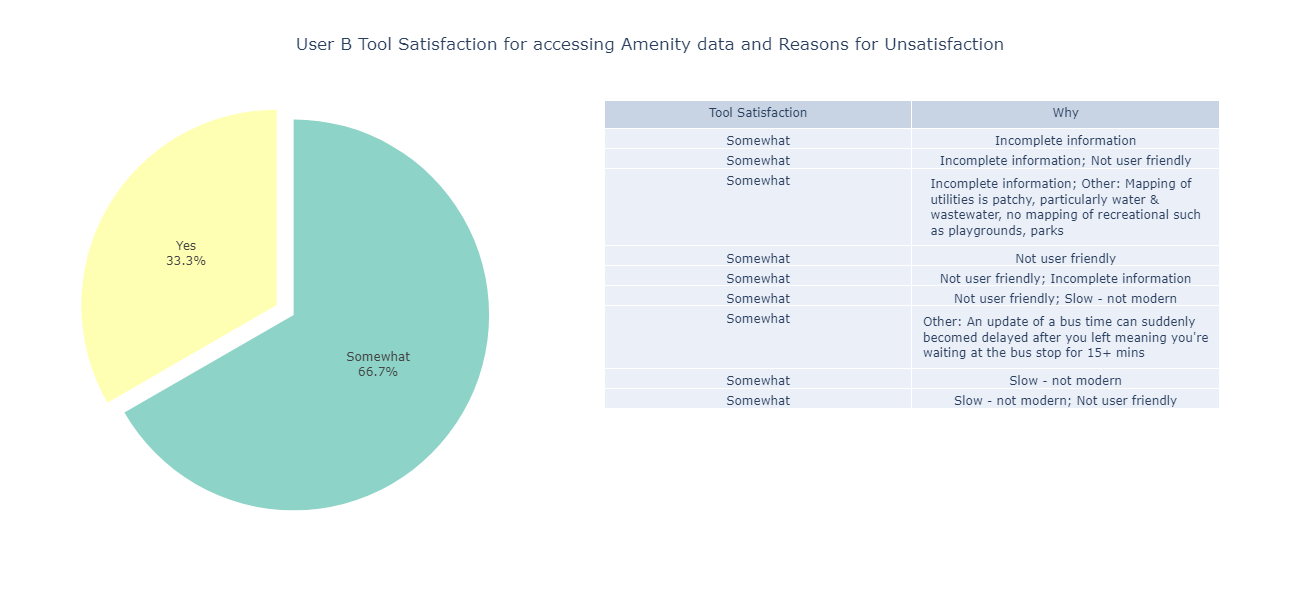
\includegraphics[width=0.8\textwidth]{images/mr-userb-tool-satisfaction.png}
    \caption{Market analysis - User B Tool satisfaction \& Usage frequency}
\end{figure}

\subsubsection{Thoughts on Magpie}
Lastly, this section covers questions regarding Magpie's potential to bridge the
gap in modern visualizing solutions.

%magpie usefulness user a
\begin{figure}[htbp]
    \centering{}
    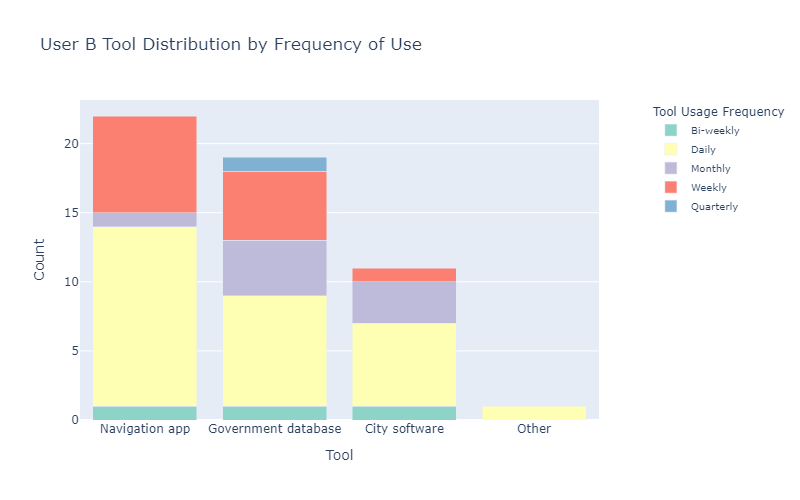
\includegraphics[width=0.8\textwidth]{images/mr-userb-tool-freq.png}
    \caption{Market analysis - User A Thoughts on Magpie}
\end{figure}

%magpie usefulness user b
\begin{figure}[htbp]
    \centering{}
    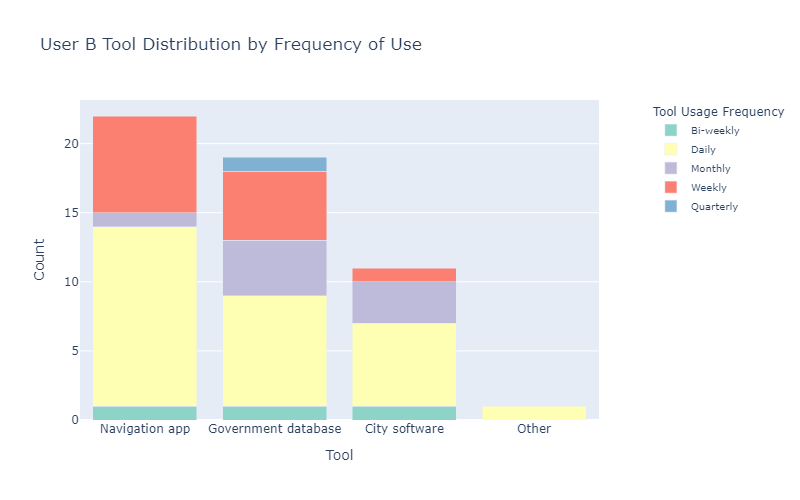
\includegraphics[width=0.8\textwidth]{images/mr-userb-tool-freq.png}
    \caption{Market analysis - User B Thoughts on Magpie}
\end{figure}

Both user groups found that Magpie would be useful to access amenity data, less
than 5\% citing it would be impractical because either they did not require
access to this information, or other tools such as Google Maps already satisfied
their needs.

Users from group B were also asked what additional features they would like to
see on Magpie. The highest rated ones were a \textbf{search functionality} and
\textbf{filters}.

%magpie usefulness user b
\begin{figure}[htbp]
    \centering{}
    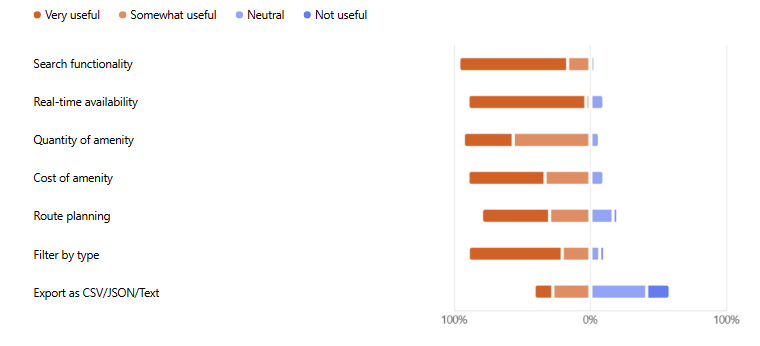
\includegraphics[width=0.8\textwidth]{images/mr-extra-features.png}
    \caption{Market analysis - User B Rating Additional Features}
\end{figure}

\textbf{Overall}, this exploratory work allows us to confirm our primary and
secondary target users as \emph{urban planners} and \emph{general users}
respectively.

Additionally, it gave us insight into a feature list to implement throughout
development, as well as competitors to research into.

\end{document}

\section{Technical Problem:}
\subsection{Why does our system exist?}
In our research, we couldn't find a singular system that allows users to gain a
general overview of public amenities, for example, parking, bike infrastructure,
or public transport. In Ireland and the United Kingdom, the prevalence of proper
digitised records in county administrations varies wildly
(\cite{WebAccessibilityIreland}). Some make use of state-of-the-art geographical
information systems (GIS) while others rely on spreadsheets which are manually
kept up to date. (\cite{mcguirk2001changing})

\noindent{}A system that would allow users to quickly inspect a combined dataset
grounded in automatically generated, real-world data could accelerate processes
like planning permissions, urban development, or resource allocation. This
applies especially to smaller counties that may not have personnel experienced
in this area. (\cite{clark2002amenities})

\noindent{}Improving how governments allocates resources could lead to
improvements in efficiency, making public services more attainable, even for
smaller communities. For example, having accurate data on public transport and
bike infrastructure encourages more people to choose sustainable modes of
transport, helping reduce carbon and noise emissions (\cite{MUGION20181566}). It
could also make it easier for people in underserved communities to access
important services, such as housing, thus helping to bridge social gaps.
(\cite{allen2015understanding})

\noindent{}Currently, solutions are fragmented, focusing on just one type of
amenity, like transport or housing, without giving a full picture. Even the more
advanced GIS systems, while powerful, usually need a lot of manual input or
additional programming, which smaller municipalities or organizations might not
be able to handle. For example, to find parking spots in an area, the user needs to
either bring their own dataset or they have to perform computer vision analysis
themselves. While \textit{ArcGIS} includes tools to run deep learning on raster
images, the process is far from straight forward. Many of these GIS tools are also
expensive, or require specialised training, making them out of reach for smaller
boroughs or counties. (\cite{kaufmann2022scaling})

\subsection{The core technical problem}
The problem at the heart of our project is to find a way to collate and
visualize useful data about public amenities, without the need for any existing
information or manual data entry. This would allow the solution to be useful, no
matter the state of the users digital records. Relying purely on existing data
would do nothing to reduce the divide between counties with more data and
counties with less data. This necessitates the creation of an interconnected
series of modules that form a pipeline, for the automatic extraction and fusion
of data.

\noindent{}In order to present users with a map containing information about the
number of public amenities, we must first identify them. Our biggest technical
challenge is the extraction of these data points. Different forms of public
amenities exist in satellite imagery, we can combine this with other data
sources, interweaving them, and producing a better result.

\noindent{}Detecting public amenities from overhead views is a non-trivial process,
as satellite imagery suffers from low resolution, occlusion, seasonal changes, or
cloud cover. This means classifying specific objects can be complicated, and can
take a lot of time and processing power. For instance, the task of quantifying
on-street parking is dependent on reliably detecting cars that are not actively
participating in traffic (in aerial images). Not only that, but the detected
points in the images must be mapped back onto real-world coordinates to be of
any utility.

\noindent{}Ensuring consistency between the extracted data, and other data sets,
can have its own pitfalls. For example, compensating for:

\vspace{-3mm}
\begin{itemize}
  \item{different precision in geographical alignment}
  \item{varied update frequencies}
  \item{different data formats}
\end{itemize}
\vspace{-3mm}

\noindent{}Not only can data be geographically misaligned, but since satellite
data is only a snapshot in time, it can lead to temporal misalignment as well.
Even the appearance of amenities can change depending on their location. While
cars look more or less the same anywhere on Earth, the same cannot be said for
public transport links, housing or hospitals, which could lead to difficulties
achieving the same level of accuracy in different regions. Processing a large
amount of data like can be difficult and finding a strategy to do this
efficiently is necessary.

\subsection{A review of similar systems}

\noindent{}\textbf{Parkopedia}

\begin{figure}[h]
  \centering
  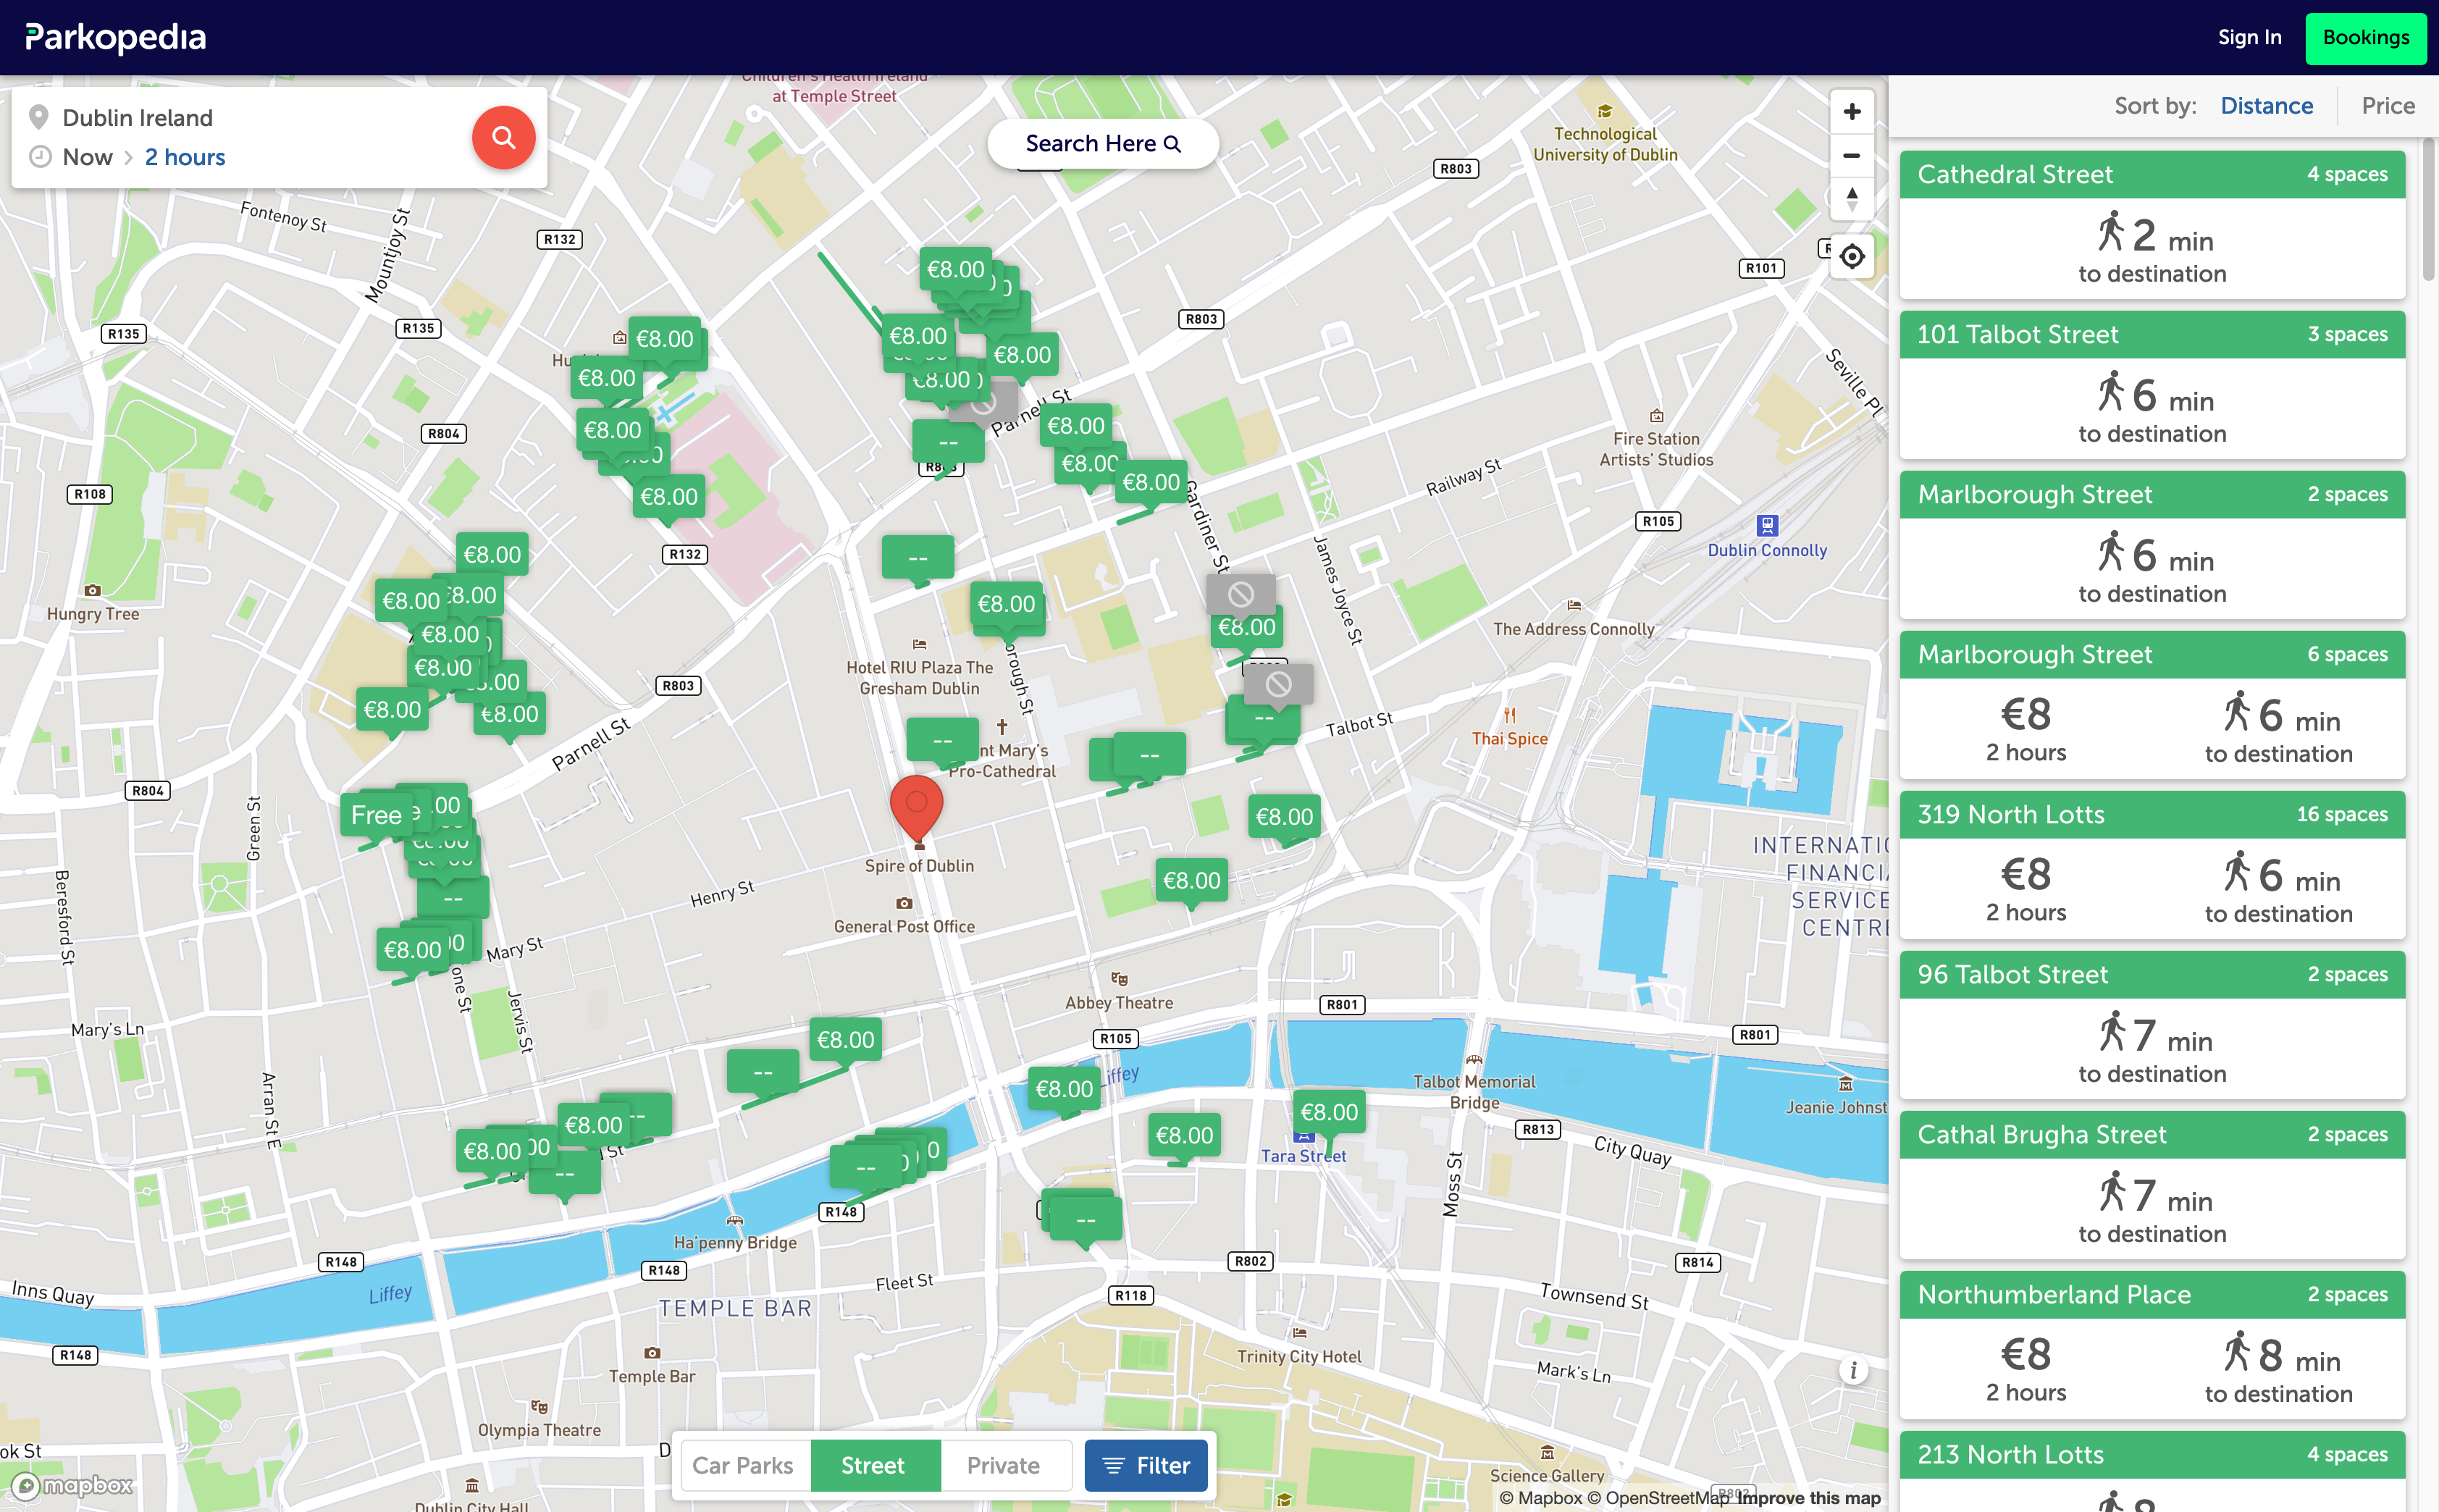
\includegraphics[width=\columnwidth]{images/parkopedia.png}
  \caption{Example of parkopedia}
  \label{fig:parkopedia}
\end{figure}

\noindent{}\textit{Parkopedia}\footnote{https://www.parkopedia.com/} is a web
application that allows users to find parking in many cities around the world.
They offer location and pricing data on parking garages, on-street parking and
parking on private property.

\noindent{}It is similar to \textit{Magpie} in the sense that it allows users to
gain a quick overview of all parking options in their area.

\noindent{}Our system differentiates itself from \textit{Parkopedia} in three
main ways:
\vspace{-3mm}
\begin{itemize}
  \item{\textbf{Data fusion:} Our system integrates data from publicly available
  sources, combining multiple datasets to provide a more comprehensive overview
  of public amenities -- not just parking.}
  \vspace{1.25mm}

  \item{\textbf{Aggregated data:} Our system offers a high-level overview of the
  amount of available amenities in a certain radius. This would be possible with
  the data from \textit{Parkopedia}, but the user would have to manually
  retrieve the data in which they are interested in analysing.}
  \vspace{1.25mm}

  \pagebreak{}

  \item{\textbf{No reliance on manual data entry:} Unlike
  \nobreak{\textit{Parkopedia}}, which relies on user-submitted information, we
  automatically acquire and fuse datasets. This pipeline allows us to keep
  information up-to-date and adapt our system to new regions without the need
  for manual data input.}
  \vspace{1.25mm}

\end{itemize}

\noindent{}\textbf{ArcGIS}

\begin{figure}[h]
  \centering
  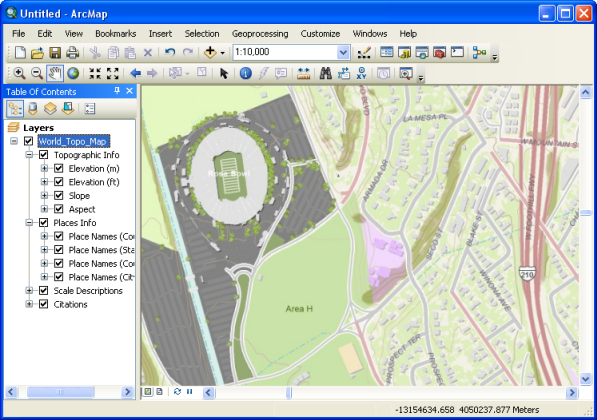
\includegraphics[width=0.85\columnwidth]{images/arcgis.png}
  \caption{Example of ArcGIS}
  \label{fig:arcgis}
\end{figure}

\noindent{}Systems like \textit{ArcGIS}\footnote{https://www.arcgis.com/} target
mainly expert users like cartographers and researchers. These systems are powerful
and feature-rich tools for professionals. While \textit{ArcGIS} is able to produce
the same overview offered by our system, it is different in these key aspects:

\begin{samepage}
\begin{itemize}
    \item{\textbf{Ease of use:} The goal of our system is to cater to a broad
    range of users, not just experts. Systems like \textit{ArcGIS} require
    specialised domain knowledge, as it's aimed at professional users. While
    \textit{ArcGIS} offers powerful tools, it can be overwhelming for the more
    general user who needs a quick overview of public amenities without engaging
    with advanced features.}
  \vspace{1.25mm}

  \item{\textbf{Accessibility:} GISs are a robust tool, but its access is often
  restricted lack of technical expertise. Compared to \textit{ArcGIS}, our
  system is less versatile. However, our system is more streamlined to offer- at
  a glance- an easily accessible way of gauging information about public
  amenities. This makes sure that users from all backgrounds can utilize our
  system without the need for specialised training.}
  \vspace{1.25mm}

\end{itemize}
\end{samepage}

% Fixes formatting
\pagebreak{}

\section{Technical Solution:}
\textbf{Technologies}

\begin{figure}[h]
  \centering
  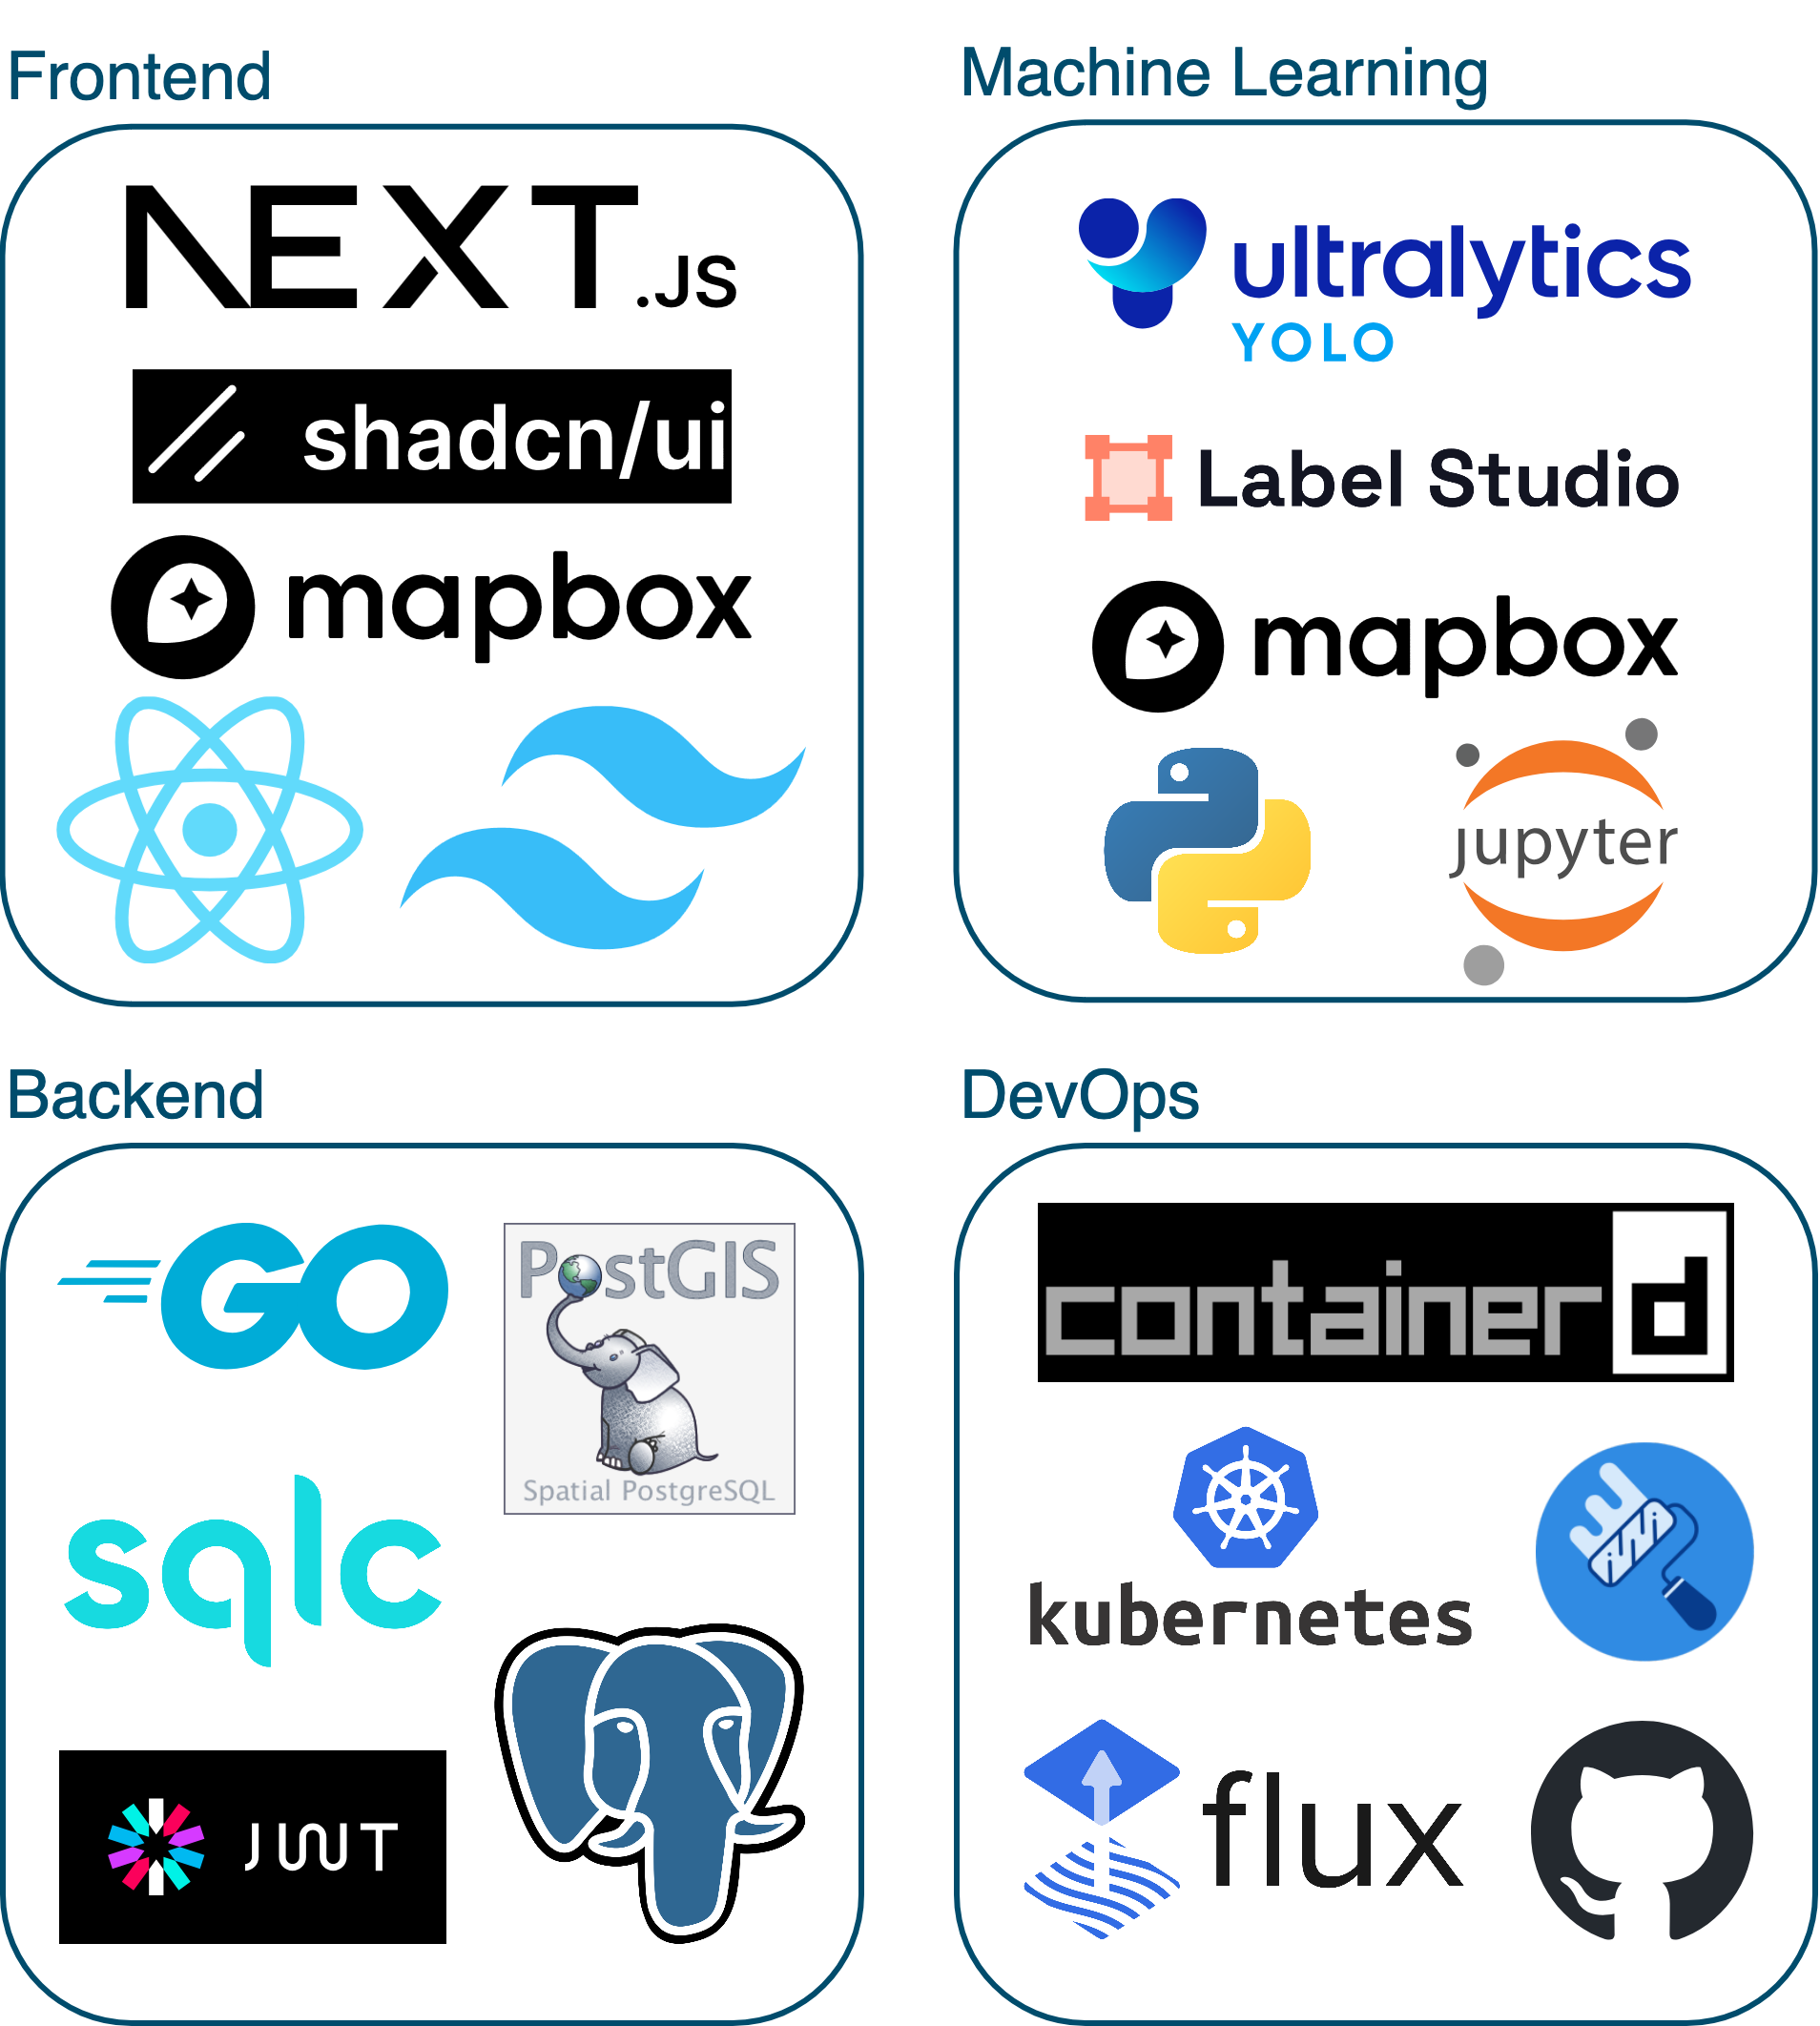
\includegraphics[width=0.8\columnwidth]{images/stack_grid.png}
  \caption{Technologies used in \textit{Magpie}}
  \label{fig:tech_stack}
\end{figure}

\subsection{Frontend}
With \textit{Magpie}, we utilized a modern web development stack, integrating
several technologies to optimize performance, scalability, and maintainability.
Below is a breakdown of the primary technologies and their roles in the project.

\vspace{-3mm}
\begin{enumerate}
    \item{\textbf{React:} React is a popular JavaScript library for building
    user interfaces, we used React in conjunction with Next.js to enable a
    component-driven architecture. This allowed for reusable UI components,
    which increased development efficiency and ensured maintainability.}
    \vspace{1.25mm}

    \item{\textbf{Next.js:} Next.js is a React Framework that offers server-side
    rendering (SSR) and static site generation (SSG), both of which are
    advantageous for optimizing load times and improving SEO. In this project,
    Next.js was used as the core frontend framework, enabling us to build a
    performant web application with powerful routing and SSR capabilities.}
    \vspace{1.25mm}

    \item{\textbf{TailwindCSS:} TailwindCSS, a utility-first CSS framework, was
    implemented for styling the application. It enabled rapid UI development by
    providing low-level utility classes, allowing us to avoid writing custom
    CSS. The addition of tailwind-merge and tailwindcss-animate facilitated more
    complex styling and animations.}
    \vspace{1.25mm}

    % Forcing a page break here to keep the list together
    \pagebreak{}

    \item{\textbf{Mapbox GL and React Map GL:} For map-based features, Mapbox GL
    and React Map GL were utilized. Mapbox GL provided the core functionality
    for interactive maps, while React Map GL integrated this into our React
    components efficiently. Deck.gl was also used for advanced visualization
    layers on top of maps, enabling us to display large data sets smoothly.}
    \vspace{1.25mm}

    \item{\textbf{ShadCN/UI:} For building UI components, we incorporated
    ShadCN, a component library designed on top of Radix Primitives. ShadCN
    brings the flexibility of Radix UI while combining it with a more
    opinionated design system, tailored specifically for projects that require
    custom styling with the power of TailwindCSS. This allowed for highly
    customizable, accessible components, with minimal configuration, speeding up
    the development process while maintaining design consistency. ShadCN’s tight
    integration with Radix Primitives helped ensure accessibility standards were
    met without sacrificing flexibility.}
    \vspace{1.25mm}

\end{enumerate}

\noindent{}The integration of these technologies into the project provided a
solid foundation for building a performant, scalable, and user-friendly web
application. From Next.js for SSR to ShadCN for accessible components, each tool
played a crucial role in achieving the project’s goals while maintaining high
standards of code quality, user experience, and performance.

\subsection{Machine Learning}

This project aims to provide a tool that allows Urban Planners to make informed
decisions using multiple data sources. Early on in the project, we identified
that on-street parking detection would be a key feature of the platform,
realising this would be the most difficult element of the machine learning
pipeline, we decided to tackle this first.

\noindent{}To detect parking spots from satellite images, the following steps
are implemented: image acquisition, mask generation, car detection, and finally
parking spot localisation.

\vspace{-3mm}
\begin{itemize}
  \item{First, satellite images and corresponding road map images are retrieved
  for a specific area contained within a bounding box, defined by its top-left
  and bottom-right coordinates, from the Mapbox API.}
  \vspace{1.25mm}

  \item{Next, a binary mask is generated by identifying road pixels based on
  their colour. The majority of roads are depicted in white, though motorways or
  major roads are marked in orange and yellow, which are detected through
  additional colour masks.}
  \vspace{1.25mm}

  % Forcing a page break here to keep the list together
  \pagebreak{}

  \item{The masks are then combined and refined using morphological operations
  to remove additional noise (street names), simplifying the image to isolate
  the roads from other elements.}
\end{itemize}

% We want to maintain paragraphs on the same page where possible \pagebreak{}

\noindent{}We train a model to recognize all cars based on images from our
dataset. We chose the YOLO (You-Only-Look-Once) model because of its popularity
and great results in the object detection task. We started with version 5 and
upgraded to version 8 for its improved accuracy.

\begin{figure}[h]
  \centering
  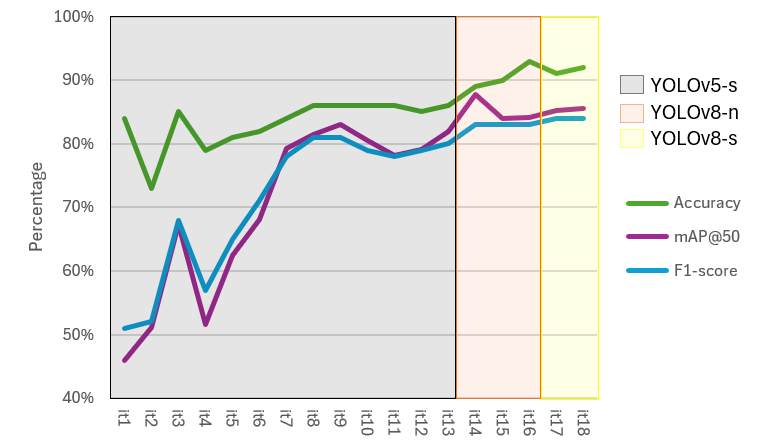
\includegraphics[width=\columnwidth]{images/training_table1.png}
  \caption{Yolo v5 vs Yolo v8 comparison}
  \label{fig:parking_detection}
\end{figure}

\noindent{}Through the training process, accuracy results stagnated caused by
labelling inconsistencies in our dataset. For example, bounding boxes were not
rotated correctly to fit the cars, thus making it harder for the model to
recognize them consistently and with confidence. After cautious re-labelling,
training continued, testing different optimizers, epoch numbers, and patience
thresholds.

\noindent{}This resulted in:
\begin{mdframed}[innerleftmargin=0pt, innerrightmargin=0pt, innertopmargin=0pt, innerbottommargin=0pt]
\begin{align*}
\text{Accuracy:} & \quad 92\% \\
\text{Precision:} & \quad 100\% \\
\text{Confidence Threshold (Precision):} & \quad 75.1\% \\
\text{Recall:} & \quad 98\% \\
\text{F1-Score:} & \quad 84\% \\
\text{mAP@50:} & \quad 85.6\% \\
\text{Optimal Confidence Threshold (F1 curve):} & \quad 35.8\%
\\
\end{align*}
\end{mdframed}

\noindent{}Next, the fine-tuned YOLOv8 model is used to detect cars in the
satellite images. The road mask is overlaid over the output of the initial model
to exclude cars on the road, resulting in a set of cars which are not on the
road, we have decided to consider these parked cars. Once the parked cars are
identified, we then convert the marked cars into coordinates.

\begin{figure}[h]
    \centering
    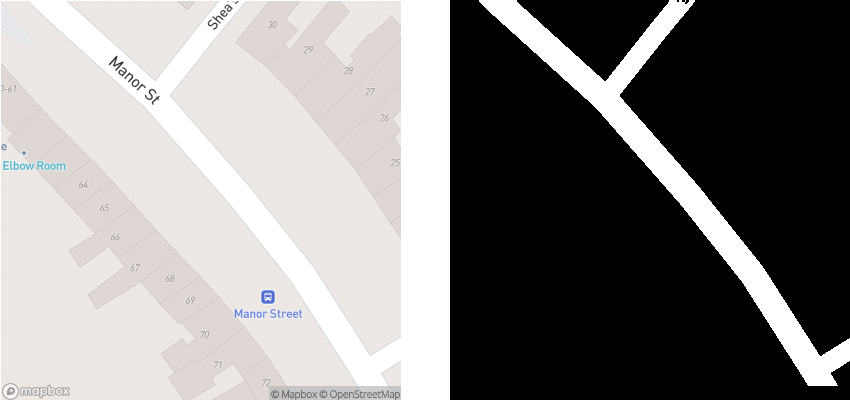
\includegraphics[width=\columnwidth]{images/mask_and_mapbox.png}
    \caption{Example of mask and mapbox image}
    \label{fig:mask_and_mapbox}
\end{figure}

\noindent{}Finally, the locations of all parking spots found within the
specified bounding box are saved in a CSV file and subsequently sent to the
PostgreSQL database.

\begin{figure}[h]
    \centering
    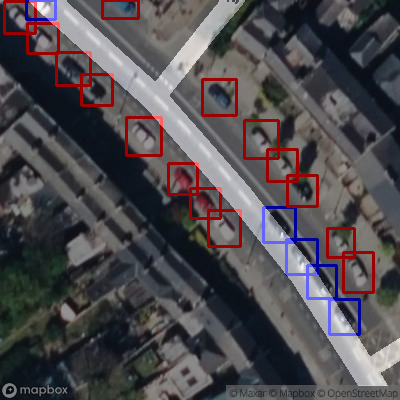
\includegraphics[width=0.65\columnwidth]{images/opacity_mask.png}
    \caption{Parking with mask applied}
    \label{fig:parking_detection}
\end{figure}

\subsection{Backend}

Supplying the data extracted by the machine learning model to the frontend is
the task of two separate backend applications. Both interact with a PostgreSQL
database, which acts as the heart of the system.

\noindent{}\textbf{Why split the backend?}

\noindent{}The backend is split into two components -- a private and a public
backend. This is achieved by utilising build tags to compile two applications
with two feature sets from a shared Golang codebase. Using a split architecture
for the backend provides two key advantages:

\vspace{-3mm}
\begin{itemize}
  \item{\textbf{Scalability:} The decision to deploy the application containers
  using Kubernetes incentivize the use of smaller services. This allows each
  component of the service to be scaled independently. Since each service will
  encounter high traffic situations under different circumstances, this
  flexibility is advantageous.}

  \item{\textbf{Security:} The private backend is strictly accessible from
  inside the cluster itself. This makes the points data essentially immutable to
  the public backend. Even if a malicious actor manages to gain elevated
  privileges on their user account, the public backend is unable to make changes
  to point data.}
\end{itemize}
\vspace{-3mm}

\begin{figure}[h]
  \centering{
  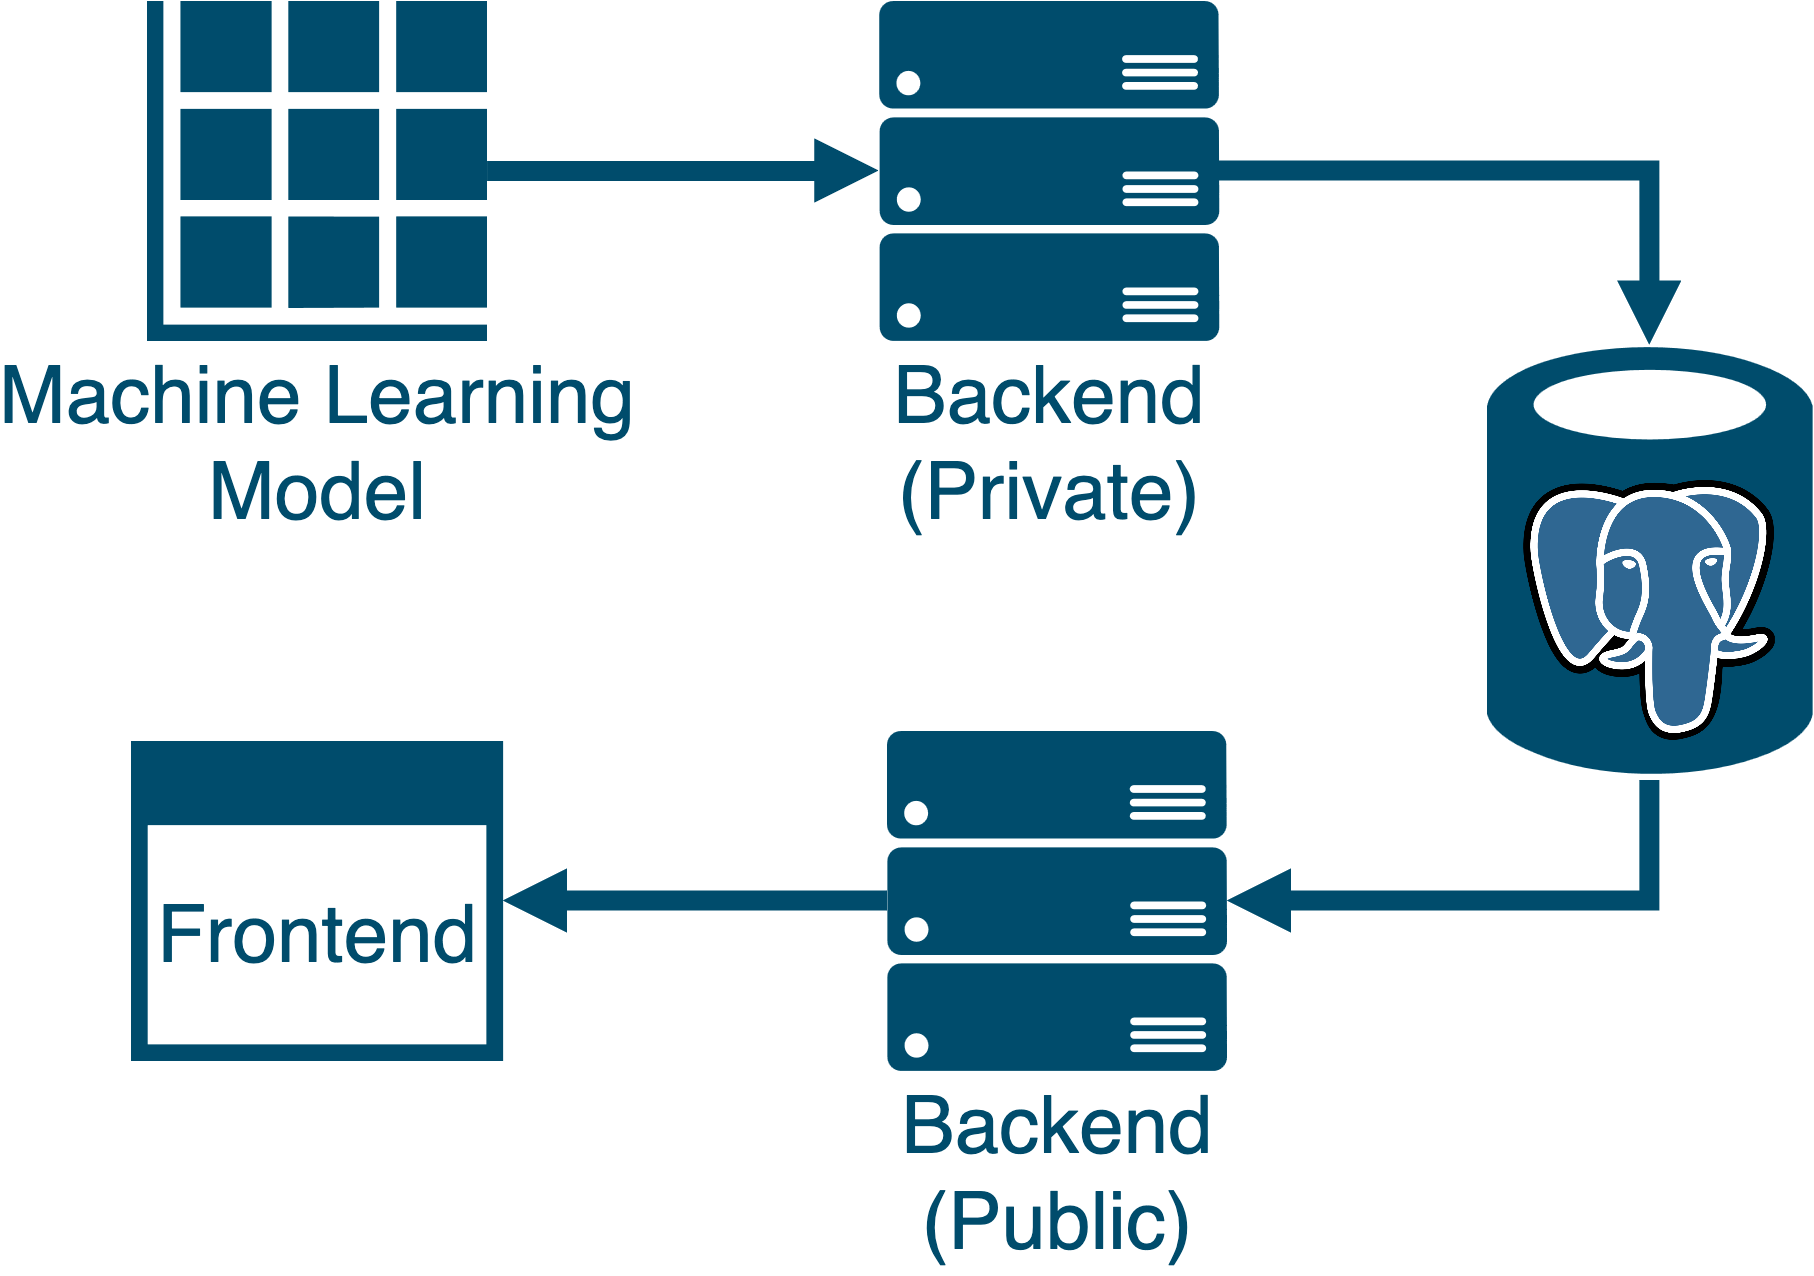
\includegraphics[width=0.80\columnwidth]{images/dataflow_backend2.png}
  \caption{Example of backend data flow}
  \label{fig:dataflow_backend2}
  }
\end{figure}

% Forcing a page break here to keep the list together
\pagebreak{}

\noindent{}\textbf{Private Backend}

\noindent{}The private backend serves as an interface between the machine
learning model and the database. It takes in the extracted datapoints via a REST
API and inserts them into the database. It is accessible strictly from IP
addresses inside the cluster.

\noindent{}\textbf{Public Backend}

\noindent{}The public backend serves as an interface between the frontend and
the database. It exposes routes to manage user accounts (CRUD) and request the
data extracted by the machine learning model (read-only).

\noindent{}The authentication is handled using JSON Web Tokens and bcrypt. Some
routes are protected depending on access level (public, logged-in, user-only).

\subsection{DevOps}

From the beginning, the \textit{Magpie} project was intended to be built as
fast, and with the least amount of friction, as possible. To achieve this, we
implemented as many DevOps strategies as we had the skill and knowledge to
implement.

\noindent{}\textbf{Kubernetes}

\noindent{}The core of our deployment strategy is Kubernetes. Kubernetes is a
container orchestration platform that allows us to deploy, scale, and manage
containerized applications. As mentioned in previous sections, designing an
application for Kubernetes grants us opportunities as well as design
considerations. For example, we can easily configure our application to load
balance- but to allow for this, we need to adopt a microservice architecture.

\noindent{}However, while Kubernetes is a great deployment tool, it can be difficult to
maintain consistency between the state of the cluster and our codebase. To solve
this we use \textit{Flux}. Flux watches a Git repository and (on an interval)
replicates the Kubernetes config to the cluster.

% Forcing a page break here to keep the list together
\pagebreak{}

\noindent{}\textbf{Continuous Integration}

\noindent{}Flux only solves half of the problem. We also need to ensure that our
containerised application is built, otherwise, while Flux will replicate the
config, it will not update the application. To solve this, we use \textit{GitHub
Actions.}. We have implemented several Actions which build the application. Once
built, the containers are pushed to the \textit{GitHub Container Registry}.

\noindent{}There are scenarios where we may have a built container but may not
want to deploy it immediately. As such, we make use of \textit{Mend Renovate}.
Renovate is a tool that automatically updates dependencies in Git repositories
by creating pull requests. Whenever we build a new version of the code, Renovate
will create a pull request to update the container version. This allows us to
keep our deployments up to date, but also allows us to manually chose
\textit{when} to update.

\section{Evaluation:}
\subsection{Definition of Success}
Our project defines success by how effective it is in addressing the identified
challenges faced by Urban Planners.

\noindent{}To gauge if \textit{Magpie} solves the problems outlined in chapter 1
and 2, the following points need to be evaluated:
\vspace{-3mm}
\begin{itemize}
  \item{\textbf{Efficient Data Aggregation:} Does \textit{Magpie} offer the user
  a comprehensive overview of multiple kinds of public amenities in a
  geographical region they selected?}
  \item{\textbf{Automatic Data Extraction:} Does \textit{Magpie} include a data
  pipeline to extract and integrate new data automatically as it becomes
  available?}
  \item{\textbf{Accuracy of Public Amenities Identification:} Are at least 80\%
  of public amenities in the dataset correctly identified and are at the most
  10\% identified incorrectly?}
  \item{\textbf{Straightforward Interface:} Does the user interface allow for
  the retrieval of desired data efficiently (measured using Click Testing,
  including metrics such as: Time Till First Click, Total Time on Task, Overall
  Number of Clicks, and Ease of Finding/Clicking)?}
  \item{\textbf{Accessibility:} Does \textit{Magpie} make a reasonable effort to
  make its user interface accessible to users with special needs?}
\end{itemize}

% Adds page break to ensure blocking
\pagebreak{}

\subsection{Code Integrity}
To guarantee the integrity of \textit{Magpie's} code, we have devised a test
strategy using automated unit tests, integration tests and end-to-end tests.

\noindent{}Unit testing allows us to do granular regression testing, alerting us
to issues before they even enter the main codebase. Integration tests offer a
surefire way to confirm that each module is compiling correctly and is ready to
be released. End-to-end tests inspect the interaction of all components,
ensuring compatibility between modules.

\noindent{}For unit tests, we aim for 100\% code coverage where practical. In
the future, we want to adopt a test-driven development workflow to prevent any
code from going untested. In the case of breaking changes, we are discussing the
use of A/B-testing or canary testing.

\subsection{CI/CD}
Using a continuous integration/continuous delivery pipeline is industry standard
and allows for rapid iteration and shorter release cycles. Our automated testing
strategy is run by the pipeline before every public release, ensuring code
integrity. Automatic building and deployment allows us to offer users a stable
software solution that is always up-to-date and regularly includes new features.

\section{Planning \& Conclusion:}
\subsection{Project Management}

\noindent{}Our project management strategy is based on the Agile methodology.
This allowed us to adapt to the changing requirements of the project
efficiently. We have divided the work into sprints, each focusing on specific
aspects of the project.

\begin{figure}[h]
    \centering{
    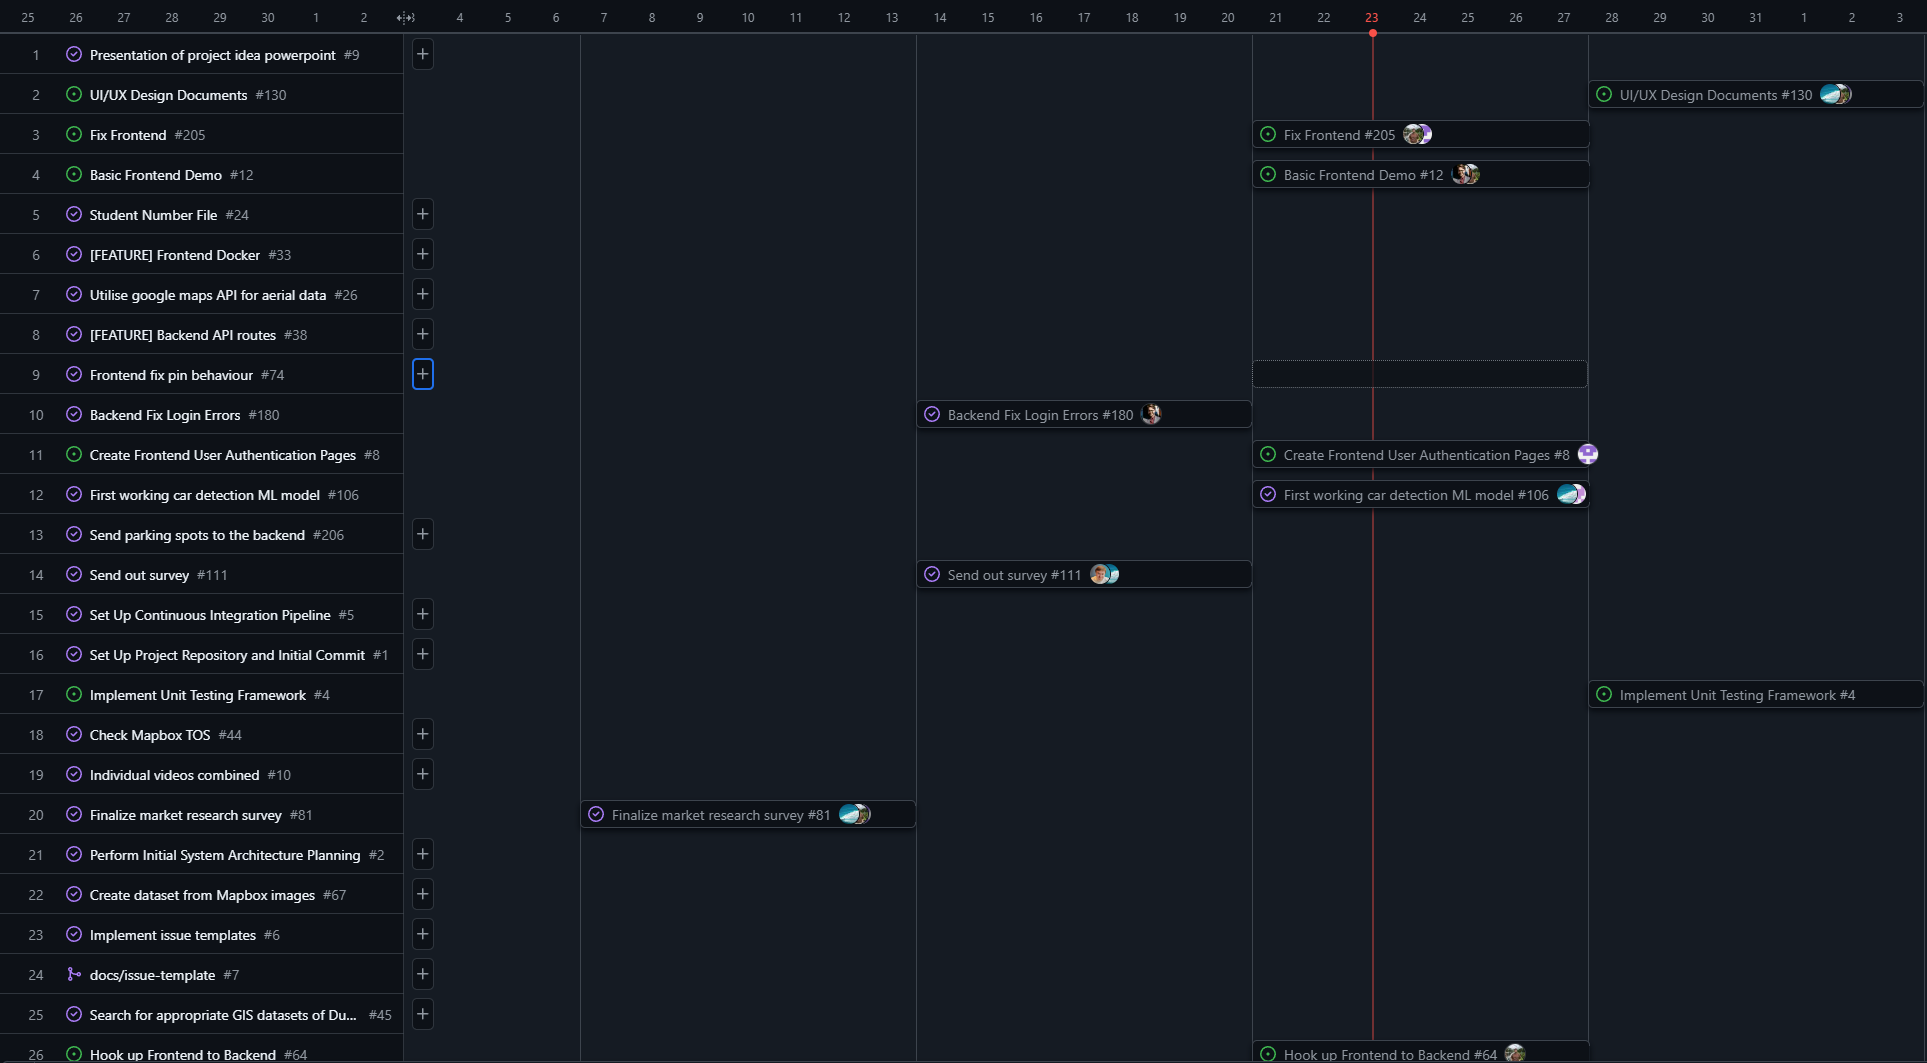
\includegraphics[width=0.95\columnwidth]{images/gantt.png}
    \caption{Section of our Gantt Chart}
    \label{fig:gantt}
  }
\end{figure}

% Adds page break to ensure blocking
\pagebreak{}

\noindent{}Daily stand-ups help maintain accountability and ensure that each
team member is aligned with the the tasks at hand that week. We are also
leveraging \textit{GitHub Projects} to track progress, set milestones and
delegate tasks efficiently across the team. We regularly perform retrospectives
to reflect on the previous weeks work and identify anything that needs to be
improved for the next week. We also perform weekly sprint planning sessions to
assign goals for that particular week, and to ensure that workload is spread
evenly across the team. Collaboration between team members is facilitated
through a \textit{Discord} server, where we can communicate and share resources.
We have setup individual channels for each section of the team to discuss
relevant topics, and remain in touch in case of issues or queries.

\begin{figure}[h]
    \centering{
    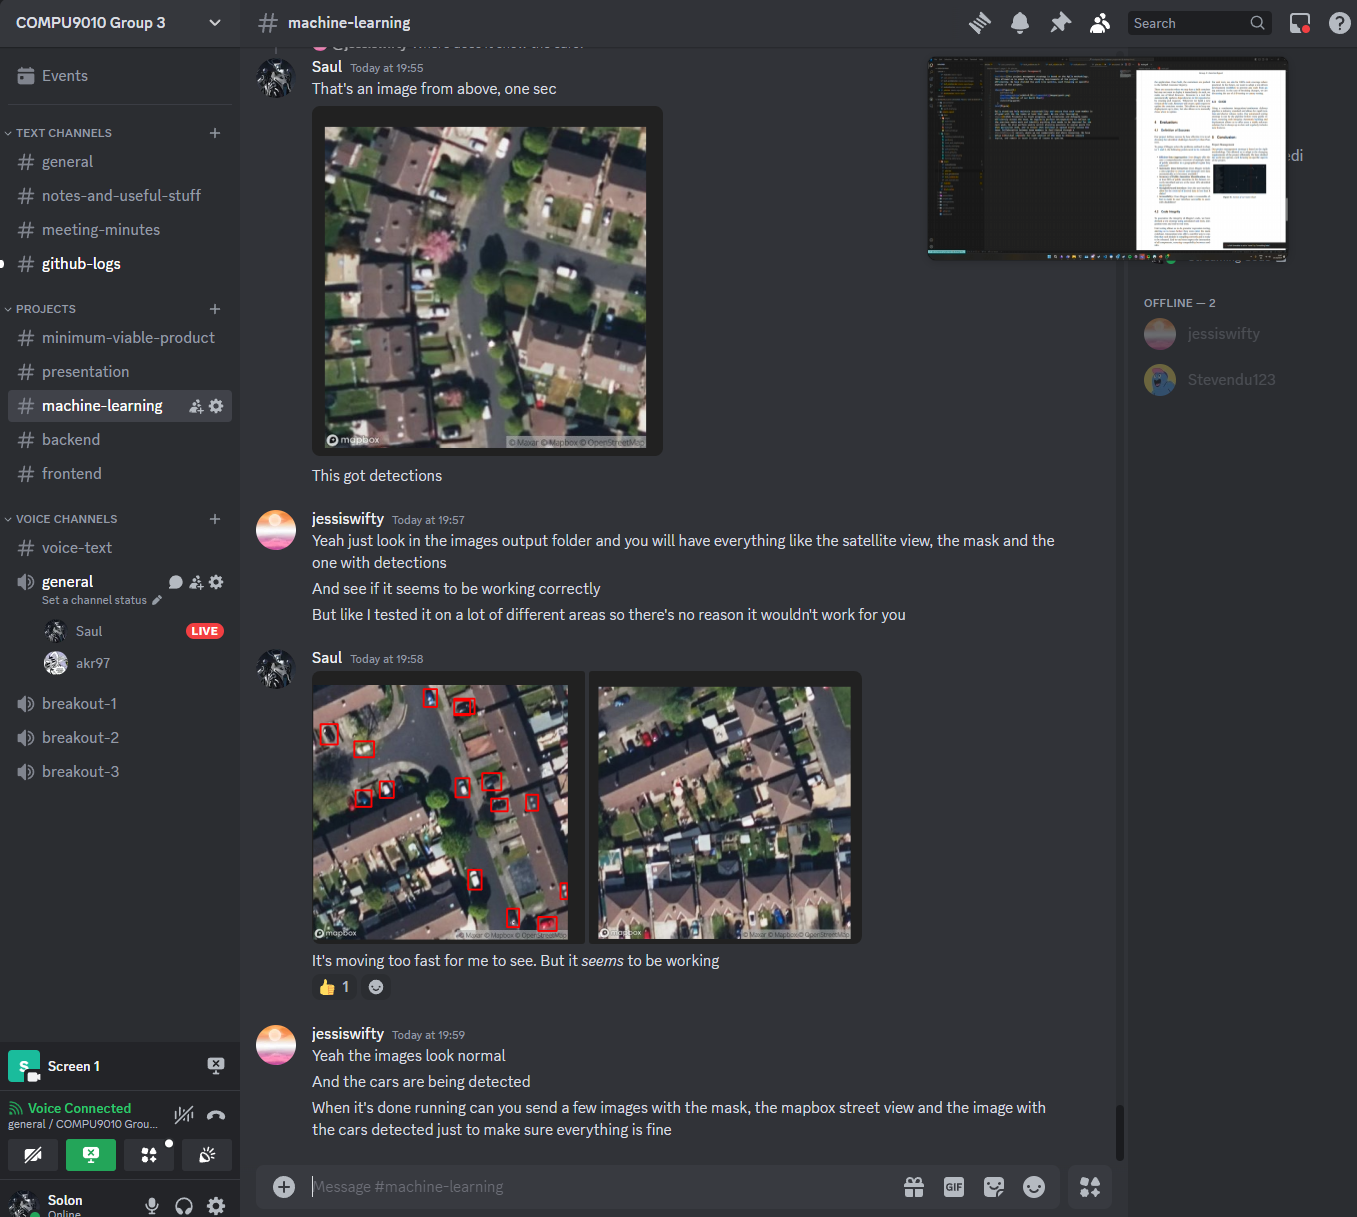
\includegraphics[width=0.95\columnwidth]{images/discord.png}
    \caption{Example of our Discord Server}
    \label{fig:discord}
  }
\end{figure}

\subsection{Current Challenges}

\noindent{}The biggest challenges we currently face include:
\vspace{-3mm}
\begin{itemize}
  \item{Ensuring detection accuracy}
  \item{Implementing additional data sources}
  \item{Improving data-pipeline}
\end{itemize}
\vspace{-3mm}

\noindent{}The current parking detection model has (in certain cases) a
propensity to misclassify some residential chimneys as parking spots. This is
due to multiple issues, for example- our satellite imagery is only precise to
20cm, and at times, the image quality is too low to distinguish the shapes. We
believe this is solvable by using masks or additional heuristics to subtract
those misclassification from the overall dataset.

\noindent{}Notably, as \textit{Magpie} is a project with low amounts of funding.
We cannot acquire higher quality data, if \textit{Magpie} were to scale, we
could also purchase satellite imagery with higher resolution. This would likely
provide enough of a difference between parking spots and chimneys to prevent
misclassification.

\noindent{}As mentioned in section 2.1, we decided to focus on parking detection
initially, as it both sets us apart from other tools, and is information that is
not easily accessible. However, a single data source would not be sufficient to meet
our goals. As such, implementing additional data sources is crucial to the overall
success of the project.

\noindent{}Early on in the project, we decided to use a \textit{Batch} process
when loading our data. We decided to take this approach for three reasons:
\vspace{-3mm}
\begin{itemize}
  \item{Reduces access required to the cluster database}
  \item{Allowed for manual checking of data before upload}
  \item{Reduced the amount of backend work}
\end{itemize}
\vspace{-3mm}

\noindent{}While none of these reasons are no longer relevant, uploading a Batch
currently requires Saul (provider of our cluster) to manually run, validate and
upload the data. While likely sustainable, this is not the \textit{best}
solution. Further investigation is needed to determine the best way of
automating this task.

\noindent{}\textbf{Plan for remaining time} To achieve a successful outcome
within the remaining timeframe, we will focus on several key priorities. 
\begin{itemize}
    \item{Firstly, we will work on optimising our parking detection model to
    enhance it's detection accuracy.}
    \\

    \item{Secondly, we will focus on implementing additional data sources. This
    will improve the overall utility of the application and provide a more
    comprehensive picture to users of avalible public amenities.}
    \\

    \item{Finally, we will work on improving the overall quality of our project.
    This will take many forms, from improving our documentation, tests, and
    code. To ensuring that \textit{Magpie} is a robust and reliable tool for our
    users.}
    \\
\end{itemize}
\vspace{-3mm}

\subsection{Conclusion}
In conclusion, \textit{Magpie} is a project that aims to provide Urban Planners
a tool that allows them to access and analyse data in a single, easy to use,
platform. To date we have achieved a number of key milestones, and provided a
minimum viable product that can be expanded to achieve our project goals.
\\ % My hatred for the necessity of this is infinite, however otherwise the formatting is off
\\
\\
\\
\\
\\
\\

% Adds page break to ensure blocking
\pagebreak{}

\begin{figure*}[h]
    \section{Appendix A: Full System Diagram:}
    \centering{
    \includegraphics[width=\textwidth]{images/System_Diagram.png}
    \caption{Full System Diagram}
    \label{fig:system_diagram}
  }
\end{figure*}

\begin{figure*}[h]
	\printbibliography[]

	\listoffigures
\end{figure*}

\end{document}
